% Capitolul 16: Recapitulare
% Statistica piețelor financiare -- Program de licență, Academia de Studii Economice din București
% GENERAT de latex/build_chapter16.py -- modificați generatorul, nu acest fișier.

\newcommand{\coursename}{Statistica piețelor financiare}
\def\sfmlang{ro}
% Preambul comun SFM -- Statistica piețelor financiare / Statistics of Financial Markets (Beamer, 16:9)
% Același design ca MFM. Înainte de % Preambul comun SFM -- Statistica piețelor financiare / Statistics of Financial Markets (Beamer, 16:9)
% Același design ca MFM. Înainte de % Preambul comun SFM -- Statistica piețelor financiare / Statistics of Financial Markets (Beamer, 16:9)
% Același design ca MFM. Înainte de \input{../../latex/preamble} se definește
%   \newcommand{\coursename}{Statistics of Financial Markets}      (EN)
%   \newcommand{\coursename}{Statistica piețelor financiare}       (RO)  și  \def\sfmlang{ro}
% Fișierele .tex se află în EN/Courses, EN/Seminars, RO/Cursuri, RO/Seminarii (două niveluri sub rădăcină).
% Deck-urile sînt generate de latex/build_chapterN.py / build_seminarN.py (vezi latex/sfm_build.py).

\documentclass[9pt, aspectratio=169, t]{beamer}
\providecommand{\coursename}{Statistics of Financial Markets}

% Ensure content fits on slides
\setbeamersize{text margin left=8mm, text margin right=8mm}

%=============================================================================
% THEME AND STYLE CONFIGURATION
%=============================================================================
\usetheme{default}
% Using default theme for clean header/footer control

% Color Palette (matching Redispatch PDF)
\definecolor{MainBlue}{RGB}{26, 58, 110}
\definecolor{AccentBlue}{RGB}{26, 58, 110}
\definecolor{IDAred}{RGB}{205, 0, 0}
\definecolor{DarkGray}{RGB}{51, 51, 51}
\definecolor{MediumGray}{RGB}{128, 128, 128}
\definecolor{LightGray}{RGB}{248, 248, 248}
\definecolor{VeryLightGray}{RGB}{235, 235, 235}
\definecolor{KeynoteGray}{RGB}{218, 218, 218}
\definecolor{SectionGray}{RGB}{120, 120, 120}
\definecolor{FooterGray}{RGB}{100, 100, 100}
\definecolor{Crimson}{RGB}{220, 53, 69}
\definecolor{Forest}{RGB}{46, 125, 50}
\definecolor{Amber}{RGB}{181, 133, 63}
\definecolor{Orange}{RGB}{230, 126, 34}
\definecolor{Purple}{RGB}{142, 68, 173}

% Gradient background (exact Keynote 315° gradient: white to RGB 218,218,218)
\setbeamertemplate{background}{%
    \begin{tikzpicture}[remember picture, overlay]
        \shade[shading=axis, shading angle=315,
        top color=white, bottom color=KeynoteGray]
        (current page.south west) rectangle (current page.north east);
    \end{tikzpicture}%
}
% Fallback solid color for compatibility
\setbeamercolor{background canvas}{bg=}

\setbeamercolor{palette primary}{bg=MainBlue, fg=white}
\setbeamercolor{palette secondary}{bg=MainBlue!85, fg=white}
\setbeamercolor{palette tertiary}{bg=MainBlue!70, fg=white}
\setbeamercolor{structure}{fg=MainBlue}
\setbeamercolor{title}{fg=IDAred}
\setbeamercolor{frametitle}{fg=IDAred, bg=}
\setbeamercolor{block title}{bg=MainBlue, fg=white}
\setbeamercolor{block body}{bg=VeryLightGray, fg=DarkGray}
\setbeamercolor{block title alerted}{bg=Crimson, fg=white}
\setbeamercolor{block body alerted}{bg=Crimson!8, fg=DarkGray}
\setbeamercolor{block title example}{bg=Forest, fg=white}
\setbeamercolor{block body example}{bg=Forest!8, fg=DarkGray}
\setbeamercolor{item}{fg=MainBlue}

% Footer colors (override Madrid theme blue)
\setbeamercolor{author in head/foot}{fg=FooterGray, bg=}
\setbeamercolor{title in head/foot}{fg=FooterGray, bg=}
\setbeamercolor{date in head/foot}{fg=FooterGray, bg=}
\setbeamercolor{section in head/foot}{fg=FooterGray, bg=}
\setbeamercolor{subsection in head/foot}{fg=FooterGray, bg=}

% Bullet styles (apply everywhere including blocks)
\setbeamertemplate{itemize item}{\color{MainBlue}$\boxdot$}
\setbeamertemplate{itemize subitem}{\color{MainBlue}$\blacktriangleright$}
\setbeamertemplate{itemize subsubitem}{\color{MainBlue}\tiny$\bullet$}
\setbeamertemplate{itemize/enumerate body begin}{\normalsize}
\setbeamertemplate{itemize/enumerate subbody begin}{\normalsize}

% Item spacing - compact style
\setlength{\leftmargini}{10pt}       % Level 1: minimal indent
\setlength{\leftmarginii}{10pt}      % Level 2: minimal additional indent
% Compact list spacing (zero extra space before/after lists in blocks)
\makeatletter
\def\@listi{\leftmargin\leftmargini \topsep 0pt \parsep 0pt \itemsep 0pt}
\def\@listii{\leftmargin\leftmarginii \topsep 0pt \parsep 0pt \itemsep 0pt}
\makeatother

\setbeamertemplate{navigation symbols}{}

%=============================================================================
% CUSTOM HEADLINE
%=============================================================================
\setbeamertemplate{headline}{%
    \vskip10pt%
    \hbox to \paperwidth{%
        \hskip0.5cm%
        {\small\color{FooterGray}\renewcommand{\hyperlink}[2]{##2}\insertsectionhead}%
        \hfill%
        \textcolor{FooterGray}{\small\insertframenumber}%
        \hskip0.5cm%
    }%
    \vskip4pt%
    {\color{FooterGray}\hrule height 0.4pt}%
}

%=============================================================================
% CUSTOM FOOTER
%=============================================================================
\usepackage{fontawesome5}

\setbeamertemplate{footline}{%
    {\color{FooterGray}\hrule height 0.4pt}%
    \vskip4pt%
    \hbox to \paperwidth{%
        \hskip0.5cm%
        \textcolor{FooterGray}{\small\coursename}%
        \hfill%
        \raisebox{-0.1em}{%
            \begin{tikzpicture}[x=0.08em, y=0.08em, line width=0.4pt]
                \draw[FooterGray] (0,3) -- (1,4) -- (2,3.5) -- (3,5) -- (4,4) -- (5,6) -- (6,5.5) -- (7,4) -- (8,5) -- (9,7) -- (10,6) -- (11,5) -- (12,6.5) -- (13,8) -- (14,7) -- (15,6) -- (16,7.5) -- (17,9) -- (18,8) -- (19,7) -- (20,8.5) -- (21,10) -- (22,9) -- (23,8) -- (24,9.5);
            \end{tikzpicture}%
        }%
        \hskip0.5cm%
    }%
    \vskip6pt%
}

%=============================================================================
% PACKAGES
%=============================================================================
\usepackage[utf8]{inputenc}
\DeclareUnicodeCharacter{03B1}{\ensuremath{\alpha}}
\usepackage[T1]{fontenc}
\usepackage{amsmath, amssymb, amsthm}
\usepackage{mathtools}
\usepackage{bm}
\usepackage{tikz}
\usetikzlibrary{arrows.meta, positioning, shapes, calc, decorations.pathreplacing, shadings}
\usepackage{booktabs}
\usepackage{multirow}
\usepackage{array}
\usepackage{graphicx}
\usepackage{hyperref}
\usepackage{colortbl}
\usepackage{listings}
\lstset{language=Python, basicstyle=\ttfamily\scriptsize, keywordstyle=\color{MainBlue}\bfseries,
  commentstyle=\color{Forest}, stringstyle=\color{Crimson}, breaklines=true,
  frame=none, backgroundcolor=\color{VeryLightGray}, xleftmargin=2mm}
\hypersetup{colorlinks=true, linkcolor=MainBlue, urlcolor=MainBlue}
\graphicspath{{../../logos/}{../../charts/}{../../photos/}}
\usepackage{xcolor}
\hfuzz=2pt  % Suppress tiny overfull warnings (<2pt)
\vfuzz=2pt  % Suppress tiny vertical overfull warnings (<2pt)

%=============================================================================
% QUANTLET COMMANDS
%   \quantlet{<displayed name>}{<url>}       (generic, compatible with the older SFM decks)
%   \sfmquantlet{Ch_05}{SFM_ch5_garch}       -> https://github.com/danpele/SFM/tree/main/Quantlets/Ch_05/SFM_ch5_garch
%   \qlurl{<folder>} is defined per chapter by the generator (Quantlets/Ch_NN/<folder>)
%=============================================================================
\newcommand{\sfmrepo}{https://github.com/danpele/SFM}
\newcommand{\sfmqlbase}{https://github.com/danpele/SFM/tree/main/Quantlets}
\newcommand{\quantlet}[2]{%
    \hfill\href{#2}{%
        \raisebox{-0.15em}{
\includegraphics[height=0.7em]{ql_logo.png}}%
        \textcolor{MainBlue}{\tiny\ #1}%
    }%
}
\newcommand{\sfmquantlet}[2]{\quantlet{\detokenize{#2}}{\sfmqlbase/#1/#2}}

%=============================================================================
% NOTEBOOKS (Google Colab)
%   \colaburl{notebooks/EN/chapter5_seminar_notebook.ipynb} -> the Colab link of a file in the SFM repo
%   \nb: the chapter notebook (each seminar deck redefines it with \renewcommand)
%=============================================================================
\newcommand{\colaburl}[1]{https://colab.research.google.com/github/danpele/SFM/blob/main/#1}
\newcommand{\nb}{https://colab.research.google.com/github/danpele/SFM/tree/main/notebooks/EN}
\newcommand{\nbname}{notebooks/EN}

%=============================================================================
% SLIDE HELPERS (used by the generators; the same as in MFM)
%=============================================================================
% local font size for list bodies (the preamble forces \normalsize)
\newcommand{\itemsize}[1]{\setbeamertemplate{itemize/enumerate body begin}{#1}\setbeamertemplate{itemize/enumerate subbody begin}{#1}}
\newcommand{\intitle}[1]{{\hypersetup{urlcolor=white}#1}}   % white links inside coloured title bars
\newcommand{\imgcap}[1]{{\scriptsize #1}\\[0.5mm]}          % caption under a photo
\newcommand{\imgcredit}[2]{{\tiny\color{FooterGray}\href{#1}{#2}}}   % image credit: source URL, author/licence
\newcommand{\aiprompt}[1]{{\ttfamily\color{MainBlue}#1}}     % a prompt to an AI assistant

%=============================================================================
% SEMINARS: student version by default; the instructor wrapper *_solutions.tex sets \solutionstrue
%=============================================================================
\makeatletter\@ifundefined{ifsolutions}{\expandafter\newif\csname ifsolutions\endcsname}{}\makeatother
\newcommand{\solonly}[1]{\ifsolutions #1\fi}
\newcommand{\propsub}{\ifsolutions\else\framesubtitle{\ifdefined\sfmlang Rezolvarea se discută la seminar\else Solution discussed in class\fi}\fi}

%=============================================================================
% APPENDIX AND CHAPTER LINKS (latex/appendix_links.py writes the calls; it also re-declares these
% macros before \begin{document}, so the decks compile with or without this preamble block)
%=============================================================================
\providecommand{\sfmapplink}[3]{\hypertarget{#2}{}\hyperlink{#1}{\beamergotobutton{#3}}}
\providecommand{\sfmappback}[2]{\begin{tikzpicture}[remember picture,overlay]\node[anchor=south east] at ([xshift=-3mm,yshift=7mm]current page.south east){\hyperlink{#1}{\beamerreturnbutton{#2}}};\end{tikzpicture}}
\providecommand{\sfmchlink}[2]{\href{#1}{#2}}
\providecommand{\sfmchlinkt}[2]{\href{#1}{\usebeamercolor[fg]{frametitle}#2}}

%=============================================================================
% QUANTINAR COMMAND: link către un curs Quantinar (subiecte avansate)
%=============================================================================
\newcommand{\quantinar}[2]{%
    \href{#2}{%
        \raisebox{-0.15em}{
\includegraphics[height=0.8em]{qr_logo.png}}%
        \textcolor{MainBlue}{\scriptsize\ #1}%
    }%
}

%=============================================================================
% CUSTOM TITLE PAGE
%=============================================================================
\defbeamertemplate*{title page}{hybrid}[1][]
{
    \vspace{0.2cm}
    % Logos row - top header (with clickable links)
    \begin{center}
        \href{https://www.ase.ro}{
\includegraphics[height=1.0cm]{ase_logo.png}}\hspace{0.3cm}%
        \href{https://theida.net}{
\includegraphics[height=1.0cm]{ida_logo.png}}\hspace{0.3cm}%
        \href{https://blockchain-research-center.com}{
\includegraphics[height=1.0cm]{brc_logo.png}}\hspace{0.3cm}%
        \href{https://www.ai4efin.ase.ro}{
\includegraphics[height=1.0cm]{ai4efin_logo.png}}\hspace{0.3cm}%
        \href{https://ipe.ro/new}{
\includegraphics[height=1.0cm]{acad_logo.png}}\hspace{0.3cm}%
        \href{https://www.digital-finance-msca.com}{
\includegraphics[height=1.0cm]{msca_logo.png}}%
    \end{center}

    \vspace{0.6cm}

    % Main title with Q logos on sides (with clickable links)
    \begin{center}
        \begin{minipage}{0.1\textwidth}
            \centering
            \href{https://quantlet.com}{
\includegraphics[height=1.1cm]{ql_logo.png}}
        \end{minipage}%
        \begin{minipage}{0.78\textwidth}
            \centering
            {\LARGE\bfseries\usebeamercolor[fg]{title}\inserttitle}

            \vspace{0.3cm}

            {\usebeamerfont{subtitle}\usebeamercolor[fg]{title}\insertsubtitle}
        \end{minipage}%
        \begin{minipage}{0.1\textwidth}
            \centering
            \href{https://quantinar.com}{
\includegraphics[height=1.1cm]{qr_logo.png}}
        \end{minipage}
    \end{center}

    \vspace{0.6cm}

    % Authors (left aligned)
    \hspace{0.5cm}{\usebeamerfont{author}\insertauthor}

    \vspace{0.3cm}

    % Institute/Affiliations (left aligned)
    \hspace{0.5cm}\begin{minipage}[t]{0.9\textwidth}
        \raggedright\small\insertinstitute
    \end{minipage}
}

%=============================================================================
% THEOREM ENVIRONMENTS
%=============================================================================
\theoremstyle{definition}
\setbeamertemplate{theorems}[numbered]
\ifdefined\sfmlang
\newtheorem{defn}{Definiție}
\newtheorem{thm}{Teoremă}
\newtheorem{prop}{Propoziție}
\newtheorem{rmk}{Observație}
\else
\newtheorem{defn}{Definition}
\newtheorem{thm}{Theorem}
\newtheorem{prop}{Proposition}
\newtheorem{rmk}{Remark}
\fi

%=============================================================================
% CENTRED MINIPAGE (no extra vertical space)
%=============================================================================
\newenvironment{cminipage}[1]{%
    \par\noindent\hfill\begin{minipage}{#1}\ignorespaces
}{%
    \end{minipage}\hfill\null\par
}

%=============================================================================
% CUSTOM COMMANDS
%=============================================================================
\newcommand{\E}{\mathbb{E}}
\newcommand{\Var}{\text{Var}}
\newcommand{\Cov}{\text{Cov}}
\newcommand{\Corr}{\text{Corr}}
\newcommand{\R}{\mathbb{R}}
\newcommand{\N}{\mathbb{N}}
\newcommand{\Z}{\mathbb{Z}}
\newcommand{\B}{\mathbf{B}}
\newcommand{\imark}{\textcolor{MainBlue}{\textbullet}}
\newcommand{\RMSE}{\text{RMSE}}
\newcommand{\MAE}{\text{MAE}}
\newcommand{\MAPE}{\text{MAPE}}

 se definește
%   \newcommand{\coursename}{Statistics of Financial Markets}      (EN)
%   \newcommand{\coursename}{Statistica piețelor financiare}       (RO)  și  \def\sfmlang{ro}
% Fișierele .tex se află în EN/Courses, EN/Seminars, RO/Cursuri, RO/Seminarii (două niveluri sub rădăcină).
% Deck-urile sînt generate de latex/build_chapterN.py / build_seminarN.py (vezi latex/sfm_build.py).

\documentclass[9pt, aspectratio=169, t]{beamer}
\providecommand{\coursename}{Statistics of Financial Markets}

% Ensure content fits on slides
\setbeamersize{text margin left=8mm, text margin right=8mm}

%=============================================================================
% THEME AND STYLE CONFIGURATION
%=============================================================================
\usetheme{default}
% Using default theme for clean header/footer control

% Color Palette (matching Redispatch PDF)
\definecolor{MainBlue}{RGB}{26, 58, 110}
\definecolor{AccentBlue}{RGB}{26, 58, 110}
\definecolor{IDAred}{RGB}{205, 0, 0}
\definecolor{DarkGray}{RGB}{51, 51, 51}
\definecolor{MediumGray}{RGB}{128, 128, 128}
\definecolor{LightGray}{RGB}{248, 248, 248}
\definecolor{VeryLightGray}{RGB}{235, 235, 235}
\definecolor{KeynoteGray}{RGB}{218, 218, 218}
\definecolor{SectionGray}{RGB}{120, 120, 120}
\definecolor{FooterGray}{RGB}{100, 100, 100}
\definecolor{Crimson}{RGB}{220, 53, 69}
\definecolor{Forest}{RGB}{46, 125, 50}
\definecolor{Amber}{RGB}{181, 133, 63}
\definecolor{Orange}{RGB}{230, 126, 34}
\definecolor{Purple}{RGB}{142, 68, 173}

% Gradient background (exact Keynote 315° gradient: white to RGB 218,218,218)
\setbeamertemplate{background}{%
    \begin{tikzpicture}[remember picture, overlay]
        \shade[shading=axis, shading angle=315,
        top color=white, bottom color=KeynoteGray]
        (current page.south west) rectangle (current page.north east);
    \end{tikzpicture}%
}
% Fallback solid color for compatibility
\setbeamercolor{background canvas}{bg=}

\setbeamercolor{palette primary}{bg=MainBlue, fg=white}
\setbeamercolor{palette secondary}{bg=MainBlue!85, fg=white}
\setbeamercolor{palette tertiary}{bg=MainBlue!70, fg=white}
\setbeamercolor{structure}{fg=MainBlue}
\setbeamercolor{title}{fg=IDAred}
\setbeamercolor{frametitle}{fg=IDAred, bg=}
\setbeamercolor{block title}{bg=MainBlue, fg=white}
\setbeamercolor{block body}{bg=VeryLightGray, fg=DarkGray}
\setbeamercolor{block title alerted}{bg=Crimson, fg=white}
\setbeamercolor{block body alerted}{bg=Crimson!8, fg=DarkGray}
\setbeamercolor{block title example}{bg=Forest, fg=white}
\setbeamercolor{block body example}{bg=Forest!8, fg=DarkGray}
\setbeamercolor{item}{fg=MainBlue}

% Footer colors (override Madrid theme blue)
\setbeamercolor{author in head/foot}{fg=FooterGray, bg=}
\setbeamercolor{title in head/foot}{fg=FooterGray, bg=}
\setbeamercolor{date in head/foot}{fg=FooterGray, bg=}
\setbeamercolor{section in head/foot}{fg=FooterGray, bg=}
\setbeamercolor{subsection in head/foot}{fg=FooterGray, bg=}

% Bullet styles (apply everywhere including blocks)
\setbeamertemplate{itemize item}{\color{MainBlue}$\boxdot$}
\setbeamertemplate{itemize subitem}{\color{MainBlue}$\blacktriangleright$}
\setbeamertemplate{itemize subsubitem}{\color{MainBlue}\tiny$\bullet$}
\setbeamertemplate{itemize/enumerate body begin}{\normalsize}
\setbeamertemplate{itemize/enumerate subbody begin}{\normalsize}

% Item spacing - compact style
\setlength{\leftmargini}{10pt}       % Level 1: minimal indent
\setlength{\leftmarginii}{10pt}      % Level 2: minimal additional indent
% Compact list spacing (zero extra space before/after lists in blocks)
\makeatletter
\def\@listi{\leftmargin\leftmargini \topsep 0pt \parsep 0pt \itemsep 0pt}
\def\@listii{\leftmargin\leftmarginii \topsep 0pt \parsep 0pt \itemsep 0pt}
\makeatother

\setbeamertemplate{navigation symbols}{}

%=============================================================================
% CUSTOM HEADLINE
%=============================================================================
\setbeamertemplate{headline}{%
    \vskip10pt%
    \hbox to \paperwidth{%
        \hskip0.5cm%
        {\small\color{FooterGray}\renewcommand{\hyperlink}[2]{##2}\insertsectionhead}%
        \hfill%
        \textcolor{FooterGray}{\small\insertframenumber}%
        \hskip0.5cm%
    }%
    \vskip4pt%
    {\color{FooterGray}\hrule height 0.4pt}%
}

%=============================================================================
% CUSTOM FOOTER
%=============================================================================
\usepackage{fontawesome5}

\setbeamertemplate{footline}{%
    {\color{FooterGray}\hrule height 0.4pt}%
    \vskip4pt%
    \hbox to \paperwidth{%
        \hskip0.5cm%
        \textcolor{FooterGray}{\small\coursename}%
        \hfill%
        \raisebox{-0.1em}{%
            \begin{tikzpicture}[x=0.08em, y=0.08em, line width=0.4pt]
                \draw[FooterGray] (0,3) -- (1,4) -- (2,3.5) -- (3,5) -- (4,4) -- (5,6) -- (6,5.5) -- (7,4) -- (8,5) -- (9,7) -- (10,6) -- (11,5) -- (12,6.5) -- (13,8) -- (14,7) -- (15,6) -- (16,7.5) -- (17,9) -- (18,8) -- (19,7) -- (20,8.5) -- (21,10) -- (22,9) -- (23,8) -- (24,9.5);
            \end{tikzpicture}%
        }%
        \hskip0.5cm%
    }%
    \vskip6pt%
}

%=============================================================================
% PACKAGES
%=============================================================================
\usepackage[utf8]{inputenc}
\DeclareUnicodeCharacter{03B1}{\ensuremath{\alpha}}
\usepackage[T1]{fontenc}
\usepackage{amsmath, amssymb, amsthm}
\usepackage{mathtools}
\usepackage{bm}
\usepackage{tikz}
\usetikzlibrary{arrows.meta, positioning, shapes, calc, decorations.pathreplacing, shadings}
\usepackage{booktabs}
\usepackage{multirow}
\usepackage{array}
\usepackage{graphicx}
\usepackage{hyperref}
\usepackage{colortbl}
\usepackage{listings}
\lstset{language=Python, basicstyle=\ttfamily\scriptsize, keywordstyle=\color{MainBlue}\bfseries,
  commentstyle=\color{Forest}, stringstyle=\color{Crimson}, breaklines=true,
  frame=none, backgroundcolor=\color{VeryLightGray}, xleftmargin=2mm}
\hypersetup{colorlinks=true, linkcolor=MainBlue, urlcolor=MainBlue}
\graphicspath{{../../logos/}{../../charts/}{../../photos/}}
\usepackage{xcolor}
\hfuzz=2pt  % Suppress tiny overfull warnings (<2pt)
\vfuzz=2pt  % Suppress tiny vertical overfull warnings (<2pt)

%=============================================================================
% QUANTLET COMMANDS
%   \quantlet{<displayed name>}{<url>}       (generic, compatible with the older SFM decks)
%   \sfmquantlet{Ch_05}{SFM_ch5_garch}       -> https://github.com/danpele/SFM/tree/main/Quantlets/Ch_05/SFM_ch5_garch
%   \qlurl{<folder>} is defined per chapter by the generator (Quantlets/Ch_NN/<folder>)
%=============================================================================
\newcommand{\sfmrepo}{https://github.com/danpele/SFM}
\newcommand{\sfmqlbase}{https://github.com/danpele/SFM/tree/main/Quantlets}
\newcommand{\quantlet}[2]{%
    \hfill\href{#2}{%
        \raisebox{-0.15em}{
\includegraphics[height=0.7em]{ql_logo.png}}%
        \textcolor{MainBlue}{\tiny\ #1}%
    }%
}
\newcommand{\sfmquantlet}[2]{\quantlet{\detokenize{#2}}{\sfmqlbase/#1/#2}}

%=============================================================================
% NOTEBOOKS (Google Colab)
%   \colaburl{notebooks/EN/chapter5_seminar_notebook.ipynb} -> the Colab link of a file in the SFM repo
%   \nb: the chapter notebook (each seminar deck redefines it with \renewcommand)
%=============================================================================
\newcommand{\colaburl}[1]{https://colab.research.google.com/github/danpele/SFM/blob/main/#1}
\newcommand{\nb}{https://colab.research.google.com/github/danpele/SFM/tree/main/notebooks/EN}
\newcommand{\nbname}{notebooks/EN}

%=============================================================================
% SLIDE HELPERS (used by the generators; the same as in MFM)
%=============================================================================
% local font size for list bodies (the preamble forces \normalsize)
\newcommand{\itemsize}[1]{\setbeamertemplate{itemize/enumerate body begin}{#1}\setbeamertemplate{itemize/enumerate subbody begin}{#1}}
\newcommand{\intitle}[1]{{\hypersetup{urlcolor=white}#1}}   % white links inside coloured title bars
\newcommand{\imgcap}[1]{{\scriptsize #1}\\[0.5mm]}          % caption under a photo
\newcommand{\imgcredit}[2]{{\tiny\color{FooterGray}\href{#1}{#2}}}   % image credit: source URL, author/licence
\newcommand{\aiprompt}[1]{{\ttfamily\color{MainBlue}#1}}     % a prompt to an AI assistant

%=============================================================================
% SEMINARS: student version by default; the instructor wrapper *_solutions.tex sets \solutionstrue
%=============================================================================
\makeatletter\@ifundefined{ifsolutions}{\expandafter\newif\csname ifsolutions\endcsname}{}\makeatother
\newcommand{\solonly}[1]{\ifsolutions #1\fi}
\newcommand{\propsub}{\ifsolutions\else\framesubtitle{\ifdefined\sfmlang Rezolvarea se discută la seminar\else Solution discussed in class\fi}\fi}

%=============================================================================
% APPENDIX AND CHAPTER LINKS (latex/appendix_links.py writes the calls; it also re-declares these
% macros before \begin{document}, so the decks compile with or without this preamble block)
%=============================================================================
\providecommand{\sfmapplink}[3]{\hypertarget{#2}{}\hyperlink{#1}{\beamergotobutton{#3}}}
\providecommand{\sfmappback}[2]{\begin{tikzpicture}[remember picture,overlay]\node[anchor=south east] at ([xshift=-3mm,yshift=7mm]current page.south east){\hyperlink{#1}{\beamerreturnbutton{#2}}};\end{tikzpicture}}
\providecommand{\sfmchlink}[2]{\href{#1}{#2}}
\providecommand{\sfmchlinkt}[2]{\href{#1}{\usebeamercolor[fg]{frametitle}#2}}

%=============================================================================
% QUANTINAR COMMAND: link către un curs Quantinar (subiecte avansate)
%=============================================================================
\newcommand{\quantinar}[2]{%
    \href{#2}{%
        \raisebox{-0.15em}{
\includegraphics[height=0.8em]{qr_logo.png}}%
        \textcolor{MainBlue}{\scriptsize\ #1}%
    }%
}

%=============================================================================
% CUSTOM TITLE PAGE
%=============================================================================
\defbeamertemplate*{title page}{hybrid}[1][]
{
    \vspace{0.2cm}
    % Logos row - top header (with clickable links)
    \begin{center}
        \href{https://www.ase.ro}{
\includegraphics[height=1.0cm]{ase_logo.png}}\hspace{0.3cm}%
        \href{https://theida.net}{
\includegraphics[height=1.0cm]{ida_logo.png}}\hspace{0.3cm}%
        \href{https://blockchain-research-center.com}{
\includegraphics[height=1.0cm]{brc_logo.png}}\hspace{0.3cm}%
        \href{https://www.ai4efin.ase.ro}{
\includegraphics[height=1.0cm]{ai4efin_logo.png}}\hspace{0.3cm}%
        \href{https://ipe.ro/new}{
\includegraphics[height=1.0cm]{acad_logo.png}}\hspace{0.3cm}%
        \href{https://www.digital-finance-msca.com}{
\includegraphics[height=1.0cm]{msca_logo.png}}%
    \end{center}

    \vspace{0.6cm}

    % Main title with Q logos on sides (with clickable links)
    \begin{center}
        \begin{minipage}{0.1\textwidth}
            \centering
            \href{https://quantlet.com}{
\includegraphics[height=1.1cm]{ql_logo.png}}
        \end{minipage}%
        \begin{minipage}{0.78\textwidth}
            \centering
            {\LARGE\bfseries\usebeamercolor[fg]{title}\inserttitle}

            \vspace{0.3cm}

            {\usebeamerfont{subtitle}\usebeamercolor[fg]{title}\insertsubtitle}
        \end{minipage}%
        \begin{minipage}{0.1\textwidth}
            \centering
            \href{https://quantinar.com}{
\includegraphics[height=1.1cm]{qr_logo.png}}
        \end{minipage}
    \end{center}

    \vspace{0.6cm}

    % Authors (left aligned)
    \hspace{0.5cm}{\usebeamerfont{author}\insertauthor}

    \vspace{0.3cm}

    % Institute/Affiliations (left aligned)
    \hspace{0.5cm}\begin{minipage}[t]{0.9\textwidth}
        \raggedright\small\insertinstitute
    \end{minipage}
}

%=============================================================================
% THEOREM ENVIRONMENTS
%=============================================================================
\theoremstyle{definition}
\setbeamertemplate{theorems}[numbered]
\ifdefined\sfmlang
\newtheorem{defn}{Definiție}
\newtheorem{thm}{Teoremă}
\newtheorem{prop}{Propoziție}
\newtheorem{rmk}{Observație}
\else
\newtheorem{defn}{Definition}
\newtheorem{thm}{Theorem}
\newtheorem{prop}{Proposition}
\newtheorem{rmk}{Remark}
\fi

%=============================================================================
% CENTRED MINIPAGE (no extra vertical space)
%=============================================================================
\newenvironment{cminipage}[1]{%
    \par\noindent\hfill\begin{minipage}{#1}\ignorespaces
}{%
    \end{minipage}\hfill\null\par
}

%=============================================================================
% CUSTOM COMMANDS
%=============================================================================
\newcommand{\E}{\mathbb{E}}
\newcommand{\Var}{\text{Var}}
\newcommand{\Cov}{\text{Cov}}
\newcommand{\Corr}{\text{Corr}}
\newcommand{\R}{\mathbb{R}}
\newcommand{\N}{\mathbb{N}}
\newcommand{\Z}{\mathbb{Z}}
\newcommand{\B}{\mathbf{B}}
\newcommand{\imark}{\textcolor{MainBlue}{\textbullet}}
\newcommand{\RMSE}{\text{RMSE}}
\newcommand{\MAE}{\text{MAE}}
\newcommand{\MAPE}{\text{MAPE}}

 se definește
%   \newcommand{\coursename}{Statistics of Financial Markets}      (EN)
%   \newcommand{\coursename}{Statistica piețelor financiare}       (RO)  și  \def\sfmlang{ro}
% Fișierele .tex se află în EN/Courses, EN/Seminars, RO/Cursuri, RO/Seminarii (două niveluri sub rădăcină).
% Deck-urile sînt generate de latex/build_chapterN.py / build_seminarN.py (vezi latex/sfm_build.py).

\documentclass[9pt, aspectratio=169, t]{beamer}
\providecommand{\coursename}{Statistics of Financial Markets}

% Ensure content fits on slides
\setbeamersize{text margin left=8mm, text margin right=8mm}

%=============================================================================
% THEME AND STYLE CONFIGURATION
%=============================================================================
\usetheme{default}
% Using default theme for clean header/footer control

% Color Palette (matching Redispatch PDF)
\definecolor{MainBlue}{RGB}{26, 58, 110}
\definecolor{AccentBlue}{RGB}{26, 58, 110}
\definecolor{IDAred}{RGB}{205, 0, 0}
\definecolor{DarkGray}{RGB}{51, 51, 51}
\definecolor{MediumGray}{RGB}{128, 128, 128}
\definecolor{LightGray}{RGB}{248, 248, 248}
\definecolor{VeryLightGray}{RGB}{235, 235, 235}
\definecolor{KeynoteGray}{RGB}{218, 218, 218}
\definecolor{SectionGray}{RGB}{120, 120, 120}
\definecolor{FooterGray}{RGB}{100, 100, 100}
\definecolor{Crimson}{RGB}{220, 53, 69}
\definecolor{Forest}{RGB}{46, 125, 50}
\definecolor{Amber}{RGB}{181, 133, 63}
\definecolor{Orange}{RGB}{230, 126, 34}
\definecolor{Purple}{RGB}{142, 68, 173}

% Gradient background (exact Keynote 315° gradient: white to RGB 218,218,218)
\setbeamertemplate{background}{%
    \begin{tikzpicture}[remember picture, overlay]
        \shade[shading=axis, shading angle=315,
        top color=white, bottom color=KeynoteGray]
        (current page.south west) rectangle (current page.north east);
    \end{tikzpicture}%
}
% Fallback solid color for compatibility
\setbeamercolor{background canvas}{bg=}

\setbeamercolor{palette primary}{bg=MainBlue, fg=white}
\setbeamercolor{palette secondary}{bg=MainBlue!85, fg=white}
\setbeamercolor{palette tertiary}{bg=MainBlue!70, fg=white}
\setbeamercolor{structure}{fg=MainBlue}
\setbeamercolor{title}{fg=IDAred}
\setbeamercolor{frametitle}{fg=IDAred, bg=}
\setbeamercolor{block title}{bg=MainBlue, fg=white}
\setbeamercolor{block body}{bg=VeryLightGray, fg=DarkGray}
\setbeamercolor{block title alerted}{bg=Crimson, fg=white}
\setbeamercolor{block body alerted}{bg=Crimson!8, fg=DarkGray}
\setbeamercolor{block title example}{bg=Forest, fg=white}
\setbeamercolor{block body example}{bg=Forest!8, fg=DarkGray}
\setbeamercolor{item}{fg=MainBlue}

% Footer colors (override Madrid theme blue)
\setbeamercolor{author in head/foot}{fg=FooterGray, bg=}
\setbeamercolor{title in head/foot}{fg=FooterGray, bg=}
\setbeamercolor{date in head/foot}{fg=FooterGray, bg=}
\setbeamercolor{section in head/foot}{fg=FooterGray, bg=}
\setbeamercolor{subsection in head/foot}{fg=FooterGray, bg=}

% Bullet styles (apply everywhere including blocks)
\setbeamertemplate{itemize item}{\color{MainBlue}$\boxdot$}
\setbeamertemplate{itemize subitem}{\color{MainBlue}$\blacktriangleright$}
\setbeamertemplate{itemize subsubitem}{\color{MainBlue}\tiny$\bullet$}
\setbeamertemplate{itemize/enumerate body begin}{\normalsize}
\setbeamertemplate{itemize/enumerate subbody begin}{\normalsize}

% Item spacing - compact style
\setlength{\leftmargini}{10pt}       % Level 1: minimal indent
\setlength{\leftmarginii}{10pt}      % Level 2: minimal additional indent
% Compact list spacing (zero extra space before/after lists in blocks)
\makeatletter
\def\@listi{\leftmargin\leftmargini \topsep 0pt \parsep 0pt \itemsep 0pt}
\def\@listii{\leftmargin\leftmarginii \topsep 0pt \parsep 0pt \itemsep 0pt}
\makeatother

\setbeamertemplate{navigation symbols}{}

%=============================================================================
% CUSTOM HEADLINE
%=============================================================================
\setbeamertemplate{headline}{%
    \vskip10pt%
    \hbox to \paperwidth{%
        \hskip0.5cm%
        {\small\color{FooterGray}\renewcommand{\hyperlink}[2]{##2}\insertsectionhead}%
        \hfill%
        \textcolor{FooterGray}{\small\insertframenumber}%
        \hskip0.5cm%
    }%
    \vskip4pt%
    {\color{FooterGray}\hrule height 0.4pt}%
}

%=============================================================================
% CUSTOM FOOTER
%=============================================================================
\usepackage{fontawesome5}

\setbeamertemplate{footline}{%
    {\color{FooterGray}\hrule height 0.4pt}%
    \vskip4pt%
    \hbox to \paperwidth{%
        \hskip0.5cm%
        \textcolor{FooterGray}{\small\coursename}%
        \hfill%
        \raisebox{-0.1em}{%
            \begin{tikzpicture}[x=0.08em, y=0.08em, line width=0.4pt]
                \draw[FooterGray] (0,3) -- (1,4) -- (2,3.5) -- (3,5) -- (4,4) -- (5,6) -- (6,5.5) -- (7,4) -- (8,5) -- (9,7) -- (10,6) -- (11,5) -- (12,6.5) -- (13,8) -- (14,7) -- (15,6) -- (16,7.5) -- (17,9) -- (18,8) -- (19,7) -- (20,8.5) -- (21,10) -- (22,9) -- (23,8) -- (24,9.5);
            \end{tikzpicture}%
        }%
        \hskip0.5cm%
    }%
    \vskip6pt%
}

%=============================================================================
% PACKAGES
%=============================================================================
\usepackage[utf8]{inputenc}
\DeclareUnicodeCharacter{03B1}{\ensuremath{\alpha}}
\usepackage[T1]{fontenc}
\usepackage{amsmath, amssymb, amsthm}
\usepackage{mathtools}
\usepackage{bm}
\usepackage{tikz}
\usetikzlibrary{arrows.meta, positioning, shapes, calc, decorations.pathreplacing, shadings}
\usepackage{booktabs}
\usepackage{multirow}
\usepackage{array}
\usepackage{graphicx}
\usepackage{hyperref}
\usepackage{colortbl}
\usepackage{listings}
\lstset{language=Python, basicstyle=\ttfamily\scriptsize, keywordstyle=\color{MainBlue}\bfseries,
  commentstyle=\color{Forest}, stringstyle=\color{Crimson}, breaklines=true,
  frame=none, backgroundcolor=\color{VeryLightGray}, xleftmargin=2mm}
\hypersetup{colorlinks=true, linkcolor=MainBlue, urlcolor=MainBlue}
\graphicspath{{../../logos/}{../../charts/}{../../photos/}}
\usepackage{xcolor}
\hfuzz=2pt  % Suppress tiny overfull warnings (<2pt)
\vfuzz=2pt  % Suppress tiny vertical overfull warnings (<2pt)

%=============================================================================
% QUANTLET COMMANDS
%   \quantlet{<displayed name>}{<url>}       (generic, compatible with the older SFM decks)
%   \sfmquantlet{Ch_05}{SFM_ch5_garch}       -> https://github.com/danpele/SFM/tree/main/Quantlets/Ch_05/SFM_ch5_garch
%   \qlurl{<folder>} is defined per chapter by the generator (Quantlets/Ch_NN/<folder>)
%=============================================================================
\newcommand{\sfmrepo}{https://github.com/danpele/SFM}
\newcommand{\sfmqlbase}{https://github.com/danpele/SFM/tree/main/Quantlets}
\newcommand{\quantlet}[2]{%
    \hfill\href{#2}{%
        \raisebox{-0.15em}{
\includegraphics[height=0.7em]{ql_logo.png}}%
        \textcolor{MainBlue}{\tiny\ #1}%
    }%
}
\newcommand{\sfmquantlet}[2]{\quantlet{\detokenize{#2}}{\sfmqlbase/#1/#2}}

%=============================================================================
% NOTEBOOKS (Google Colab)
%   \colaburl{notebooks/EN/chapter5_seminar_notebook.ipynb} -> the Colab link of a file in the SFM repo
%   \nb: the chapter notebook (each seminar deck redefines it with \renewcommand)
%=============================================================================
\newcommand{\colaburl}[1]{https://colab.research.google.com/github/danpele/SFM/blob/main/#1}
\newcommand{\nb}{https://colab.research.google.com/github/danpele/SFM/tree/main/notebooks/EN}
\newcommand{\nbname}{notebooks/EN}

%=============================================================================
% SLIDE HELPERS (used by the generators; the same as in MFM)
%=============================================================================
% local font size for list bodies (the preamble forces \normalsize)
\newcommand{\itemsize}[1]{\setbeamertemplate{itemize/enumerate body begin}{#1}\setbeamertemplate{itemize/enumerate subbody begin}{#1}}
\newcommand{\intitle}[1]{{\hypersetup{urlcolor=white}#1}}   % white links inside coloured title bars
\newcommand{\imgcap}[1]{{\scriptsize #1}\\[0.5mm]}          % caption under a photo
\newcommand{\imgcredit}[2]{{\tiny\color{FooterGray}\href{#1}{#2}}}   % image credit: source URL, author/licence
\newcommand{\aiprompt}[1]{{\ttfamily\color{MainBlue}#1}}     % a prompt to an AI assistant

%=============================================================================
% SEMINARS: student version by default; the instructor wrapper *_solutions.tex sets \solutionstrue
%=============================================================================
\makeatletter\@ifundefined{ifsolutions}{\expandafter\newif\csname ifsolutions\endcsname}{}\makeatother
\newcommand{\solonly}[1]{\ifsolutions #1\fi}
\newcommand{\propsub}{\ifsolutions\else\framesubtitle{\ifdefined\sfmlang Rezolvarea se discută la seminar\else Solution discussed in class\fi}\fi}

%=============================================================================
% APPENDIX AND CHAPTER LINKS (latex/appendix_links.py writes the calls; it also re-declares these
% macros before \begin{document}, so the decks compile with or without this preamble block)
%=============================================================================
\providecommand{\sfmapplink}[3]{\hypertarget{#2}{}\hyperlink{#1}{\beamergotobutton{#3}}}
\providecommand{\sfmappback}[2]{\begin{tikzpicture}[remember picture,overlay]\node[anchor=south east] at ([xshift=-3mm,yshift=7mm]current page.south east){\hyperlink{#1}{\beamerreturnbutton{#2}}};\end{tikzpicture}}
\providecommand{\sfmchlink}[2]{\href{#1}{#2}}
\providecommand{\sfmchlinkt}[2]{\href{#1}{\usebeamercolor[fg]{frametitle}#2}}

%=============================================================================
% QUANTINAR COMMAND: link către un curs Quantinar (subiecte avansate)
%=============================================================================
\newcommand{\quantinar}[2]{%
    \href{#2}{%
        \raisebox{-0.15em}{
\includegraphics[height=0.8em]{qr_logo.png}}%
        \textcolor{MainBlue}{\scriptsize\ #1}%
    }%
}

%=============================================================================
% CUSTOM TITLE PAGE
%=============================================================================
\defbeamertemplate*{title page}{hybrid}[1][]
{
    \vspace{0.2cm}
    % Logos row - top header (with clickable links)
    \begin{center}
        \href{https://www.ase.ro}{
\includegraphics[height=1.0cm]{ase_logo.png}}\hspace{0.3cm}%
        \href{https://theida.net}{
\includegraphics[height=1.0cm]{ida_logo.png}}\hspace{0.3cm}%
        \href{https://blockchain-research-center.com}{
\includegraphics[height=1.0cm]{brc_logo.png}}\hspace{0.3cm}%
        \href{https://www.ai4efin.ase.ro}{
\includegraphics[height=1.0cm]{ai4efin_logo.png}}\hspace{0.3cm}%
        \href{https://ipe.ro/new}{
\includegraphics[height=1.0cm]{acad_logo.png}}\hspace{0.3cm}%
        \href{https://www.digital-finance-msca.com}{
\includegraphics[height=1.0cm]{msca_logo.png}}%
    \end{center}

    \vspace{0.6cm}

    % Main title with Q logos on sides (with clickable links)
    \begin{center}
        \begin{minipage}{0.1\textwidth}
            \centering
            \href{https://quantlet.com}{
\includegraphics[height=1.1cm]{ql_logo.png}}
        \end{minipage}%
        \begin{minipage}{0.78\textwidth}
            \centering
            {\LARGE\bfseries\usebeamercolor[fg]{title}\inserttitle}

            \vspace{0.3cm}

            {\usebeamerfont{subtitle}\usebeamercolor[fg]{title}\insertsubtitle}
        \end{minipage}%
        \begin{minipage}{0.1\textwidth}
            \centering
            \href{https://quantinar.com}{
\includegraphics[height=1.1cm]{qr_logo.png}}
        \end{minipage}
    \end{center}

    \vspace{0.6cm}

    % Authors (left aligned)
    \hspace{0.5cm}{\usebeamerfont{author}\insertauthor}

    \vspace{0.3cm}

    % Institute/Affiliations (left aligned)
    \hspace{0.5cm}\begin{minipage}[t]{0.9\textwidth}
        \raggedright\small\insertinstitute
    \end{minipage}
}

%=============================================================================
% THEOREM ENVIRONMENTS
%=============================================================================
\theoremstyle{definition}
\setbeamertemplate{theorems}[numbered]
\ifdefined\sfmlang
\newtheorem{defn}{Definiție}
\newtheorem{thm}{Teoremă}
\newtheorem{prop}{Propoziție}
\newtheorem{rmk}{Observație}
\else
\newtheorem{defn}{Definition}
\newtheorem{thm}{Theorem}
\newtheorem{prop}{Proposition}
\newtheorem{rmk}{Remark}
\fi

%=============================================================================
% CENTRED MINIPAGE (no extra vertical space)
%=============================================================================
\newenvironment{cminipage}[1]{%
    \par\noindent\hfill\begin{minipage}{#1}\ignorespaces
}{%
    \end{minipage}\hfill\null\par
}

%=============================================================================
% CUSTOM COMMANDS
%=============================================================================
\newcommand{\E}{\mathbb{E}}
\newcommand{\Var}{\text{Var}}
\newcommand{\Cov}{\text{Cov}}
\newcommand{\Corr}{\text{Corr}}
\newcommand{\R}{\mathbb{R}}
\newcommand{\N}{\mathbb{N}}
\newcommand{\Z}{\mathbb{Z}}
\newcommand{\B}{\mathbf{B}}
\newcommand{\imark}{\textcolor{MainBlue}{\textbullet}}
\newcommand{\RMSE}{\text{RMSE}}
\newcommand{\MAE}{\text{MAE}}
\newcommand{\MAPE}{\text{MAPE}}



\newcommand{\qlurl}[1]{https://github.com/danpele/SFM/tree/main/Quantlets/Ch_16/#1}

% Clickable citations (DOIs verified via Crossref)

\newcommand{\refFHH}{\href{https://doi.org/10.1007/978-3-030-13751-9}{Franke, Härdle \& Hafner (2019)}}
\newcommand{\refBHL}{\href{https://doi.org/10.1007/978-3-642-33929-5}{Borak, Härdle \& López-Cabrera (2013)}}
\newcommand{\refTsay}{\href{https://doi.org/10.1002/9780470644560}{Tsay (2010)}}
\newcommand{\refCLM}{\href{https://doi.org/10.1515/9781400830213}{Campbell, Lo \& MacKinlay (1997)}}
\newcommand{\refQRM}{\href{https://press.princeton.edu/books/hardcover/9780691166278/quantitative-risk-management}{McNeil, Frey \& Embrechts (2015)}}
\newcommand{\refCont}{\href{https://doi.org/10.1080/713665670}{Cont (2001)}}
\newcommand{\refMandelbrot}{\href{https://doi.org/10.1086/294632}{Mandelbrot (1963)}}
\newcommand{\refNolan}{\href{https://doi.org/10.1007/978-3-030-52915-4}{Nolan (2020)}}
\newcommand{\refJB}{\href{https://doi.org/10.1016/0165-1765(80)90024-5}{Jarque \& Bera (1980)}}
\newcommand{\refHill}{\href{https://doi.org/10.1214/aos/1176343247}{Hill (1975)}}
\newcommand{\refFama}{\href{https://doi.org/10.2307/2325486}{Fama (1970)}}
\newcommand{\refLM}{\href{https://doi.org/10.1093/rfs/1.1.41}{Lo \& MacKinlay (1988)}}
\newcommand{\refEngle}{\href{https://doi.org/10.2307/1912773}{Engle (1982)}}
\newcommand{\refBoll}{\href{https://doi.org/10.1016/0304-4076(86)90063-1}{Bollerslev (1986)}}
\newcommand{\refRM}{\href{https://www.msci.com/documents/10199/5915b101-4206-4ba0-aee2-3449d5c7e95a}{J.P.\ Morgan/Reuters (1996)}}
\newcommand{\refArtzner}{\href{https://doi.org/10.1111/1467-9965.00068}{Artzner et al.\ (1999)}}
\newcommand{\refKupiec}{\href{https://doi.org/10.3905/jod.1995.407942}{Kupiec (1995)}}
\newcommand{\refHurst}{\href{https://doi.org/10.1061/TACEAT.0006518}{Hurst (1951)}}
\newcommand{\refPeters}{\href{https://www.wiley.com/en-us/Fractal+Market+Analysis\%3A+Applying+Chaos+Theory+to+Investment+and+Economics-p-9780471585244}{Peters (1994)}}
\newcommand{\refAltman}{\href{https://doi.org/10.1111/j.1540-6261.1968.tb00843.x}{Altman (1968)}}
\newcommand{\refGKX}{\href{https://doi.org/10.1093/rfs/hhaa009}{Gu, Kelly \& Xiu (2020)}}
\newcommand{\refNakamoto}{\href{https://bitcoin.org/bitcoin.pdf}{Nakamoto (2008)}}
\newcommand{\refAB}{\href{https://doi.org/10.1257/aer.20120555}{Adrian \& Brunnermeier (2016)}}
\newcommand{\refDY}{\href{https://doi.org/10.1016/j.ijforecast.2011.02.006}{Diebold \& Yilmaz (2012)}}
\newcommand{\refMenk}{\href{https://doi.org/10.1111/jofi.13337}{Menkveld et al.\ (2024)}}
\newcommand{\refWang}{\href{https://doi.org/10.1038/s41586-023-06221-2}{Wang et al.\ (2023)}}

\title[Statistica piețelor financiare]{Statistica piețelor financiare}
\subtitle{Capitolul 16: Recapitulare}
\author[D.T. Pele]{Daniel Traian PELE}
\institute{Academia de Studii Economice din București\\
IDA Institute Digital Assets\\
Blockchain Research Center\\
AI4EFin Artificial Intelligence for Energy Finance\\
Academia Română, Institutul de Prognoză Economică\\
MSCA Digital Finance}
\date{}

%=============================================================================
\providecommand{\sfmapplink}[3]{\hypertarget{#2}{}\hyperlink{#1}{\beamergotobutton{#3}}}  % APPLINKS-MACROS
\providecommand{\sfmappback}[2]{\begin{tikzpicture}[remember picture,overlay]\node[anchor=south east] at ([xshift=-3mm,yshift=7mm]current page.south east){\hyperlink{#1}{\beamerreturnbutton{#2}}};\end{tikzpicture}}  % APPLINKS-MACROS
\providecommand{\sfmchlink}[2]{\href{#1}{#2}}  % APPLINKS-MACROS
\providecommand{\sfmchlinkt}[2]{\href{#1}{\usebeamercolor[fg]{frametitle}#2}}  % APPLINKS-MACROS
\begin{document}
%=============================================================================

{
\setbeamertemplate{headline}{}
\setbeamertemplate{footline}{}
\begin{frame}[noframenumbering]
    \titlepage
\end{frame}
}
% BEGIN-ACRONYMS (generat de latex/acronyms.py; nu editati manual)
\begin{frame}{Acronime folosite în acest material (1/2)}
\setbeamertemplate{itemize/enumerate body begin}{\tiny}
\begin{columns}[T]
\begin{column}{0.49\textwidth}
\begin{itemize}\setlength{\itemsep}{0pt}
    \item \textbf{ACF}: Autocorrelation Function (funcția de autocorelație)
    \item \textbf{AD}: Anderson–Darling (test) — testul Anderson–Darling
    \item \textbf{AI}: Artificial Intelligence (inteligență artificială)
    \item \textbf{AIC}: Akaike Information Criterion (criteriul informațional Akaike)
    \item \textbf{ARCH}: AutoRegressive Conditional Heteroskedasticity (heteroscedasticitate condiționată autoregresivă)
    \item \textbf{ARCH-LM}: ARCH Lagrange Multiplier (test) — testul multiplicatorului Lagrange pentru efecte ARCH
    \item \textbf{AUC}: Area Under the (ROC) Curve (aria de sub curba ROC)
    \item \textbf{BET}: Bucharest Exchange Trading (index) — indicele de referință al Bursei de Valori București
    \item \textbf{BIC}: Bayesian Information Criterion (criteriul informațional bayesian)
    \item \textbf{CAGR}: Compound Annual Growth Rate (rata anuală compusă de creștere)
    \item \textbf{CI}: Confidence Interval (interval de încredere)
    \item \textbf{DFA}: Detrended Fluctuation Analysis (analiza fluctuațiilor fără tendință)
    \item \textbf{EAD}: Exposure At Default (expunerea la momentul nerambursării)
\end{itemize}
\end{column}
\begin{column}{0.49\textwidth}
\begin{itemize}\setlength{\itemsep}{0pt}
    \item \textbf{EGARCH}: Exponential GARCH (GARCH exponențial)
    \item \textbf{EODHD}: EOD Historical Data (market-data provider) — furnizor de date de piață
    \item \textbf{ES}: Expected Shortfall (pierderea așteptată în coadă)
    \item \textbf{EVT}: Extreme Value Theory (teoria valorilor extreme)
    \item \textbf{EWMA}: Exponentially Weighted Moving Average (medie mobilă ponderată exponențial)
    \item \textbf{FHS}: Filtered Historical Simulation (simularea istorică filtrată)
    \item \textbf{FPR}: False Positive Rate (rata fals pozitivelor)
    \item \textbf{GARCH}: Generalised AutoRegressive Conditional Heteroskedasticity (heteroscedasticitate condiționată autoregresivă generalizată)
    \item \textbf{GBM}: Geometric Brownian Motion (mișcarea browniană geometrică)
    \item \textbf{GEV}: Generalised Extreme Value (distribution) — distribuția generalizată a valorilor extreme
    \item \textbf{GJR}: Glosten–Jagannathan–Runkle (asymmetric GARCH) — modelul GARCH asimetric Glosten–Jagannathan–Runkle
    \item \textbf{GPD}: Generalised Pareto Distribution (distribuția Pareto generalizată)
    \item \textbf{GPH}: Geweke–Porter-Hudak (log-periodogram estimator) — estimatorul Geweke–Porter-Hudak pe log-periodogramă
\end{itemize}
\end{column}
\end{columns}
\end{frame}
\begin{frame}{Acronime folosite în acest material (2/2)}
\setbeamertemplate{itemize/enumerate body begin}{\tiny}
\begin{columns}[T]
\begin{column}{0.49\textwidth}
\begin{itemize}\setlength{\itemsep}{0pt}
    \item \textbf{HAR}: Heterogeneous AutoRegressive (model) — model autoregresiv heterogen
    \item \textbf{HS}: Historical Simulation (simularea istorică)
    \item \textbf{IGARCH}: Integrated GARCH (GARCH integrat)
    \item \textbf{JB}: Jarque–Bera (test) — testul de normalitate Jarque–Bera
    \item \textbf{KS}: Kolmogorov–Smirnov (test) — testul Kolmogorov–Smirnov
    \item \textbf{LDA}: Linear Discriminant Analysis (analiza discriminantă liniară)
    \item \textbf{LGD}: Loss Given Default (pierderea în caz de nerambursare)
    \item \textbf{LR}: Likelihood Ratio (raportul de verosimilitate)
    \item \textbf{MDD}: Maximum DrawDown (drawdown maxim)
    \item \textbf{MES}: Marginal Expected Shortfall (pierderea marginală așteptată în coadă)
    \item \textbf{NIG}: Normal Inverse Gaussian (distribution) — distribuția Normală invers Gaussiană
    \item \textbf{PD}: Probability of Default (probabilitatea de nerambursare)
    \item \textbf{QLIKE}: Quasi-LIKElihood (loss function) — funcția de pierdere de tip cvasi-verosimilitate
\end{itemize}
\end{column}
\begin{column}{0.49\textwidth}
\begin{itemize}\setlength{\itemsep}{0pt}
    \item \textbf{QQ}: Quantile–Quantile (plot) — graficul cuantilă–cuantilă
    \item \textbf{SE}: Standard Error (eroare standard)
    \item \textbf{SR}: Sharpe Ratio (raportul Sharpe)
    \item \textbf{SRISK}: Systemic RISK (capital shortfall in a crisis) — deficitul de capital într-o criză
    \item \textbf{TPR}: True Positive Rate (rata adevărat pozitivelor (sensibilitatea))
    \item \textbf{VR}: Variance Ratio (raportul varianțelor)
\end{itemize}
\end{column}
\end{columns}
\end{frame}
% END-ACRONYMS

\begin{frame}{Întrebarea de azi și traseul}
\itemsize{\small}
\begin{columns}[T]
\begin{column}{0.58\textwidth}
\begin{itemize}
    \item \textbf{Întrebarea}: ce spune întregul curs despre randamentele BET, S\&P 500 și Bitcoin și cum se evaluează aceste cunoștințe la examen?
    \begin{itemize}
        \item un capitol care leagă \sfmchlink{https://danpele.github.io/SFM/RO/Cursuri/capitol0_introducere.pdf}{Capitolele 0}--\sfmchlink{https://danpele.github.io/SFM/RO/Cursuri/capitol15_risc_sistemic.pdf}{15}
    \end{itemize}
    \item \textbf{Traseul}
    \begin{itemize}
        \item Partea I: harta cursului, cîte două slide-uri de recapitulare pentru fiecare capitol, trusa de teste și modele
        \item Partea a II-a: examenul (format, criterii de notare, opt probleme rezolvate) și proiectul de echipă
        \item Partea a III-a: contribuția posibilă a AI în propria cercetare
    \end{itemize}
\end{itemize}
\end{column}
\begin{column}{0.38\textwidth}
\centering
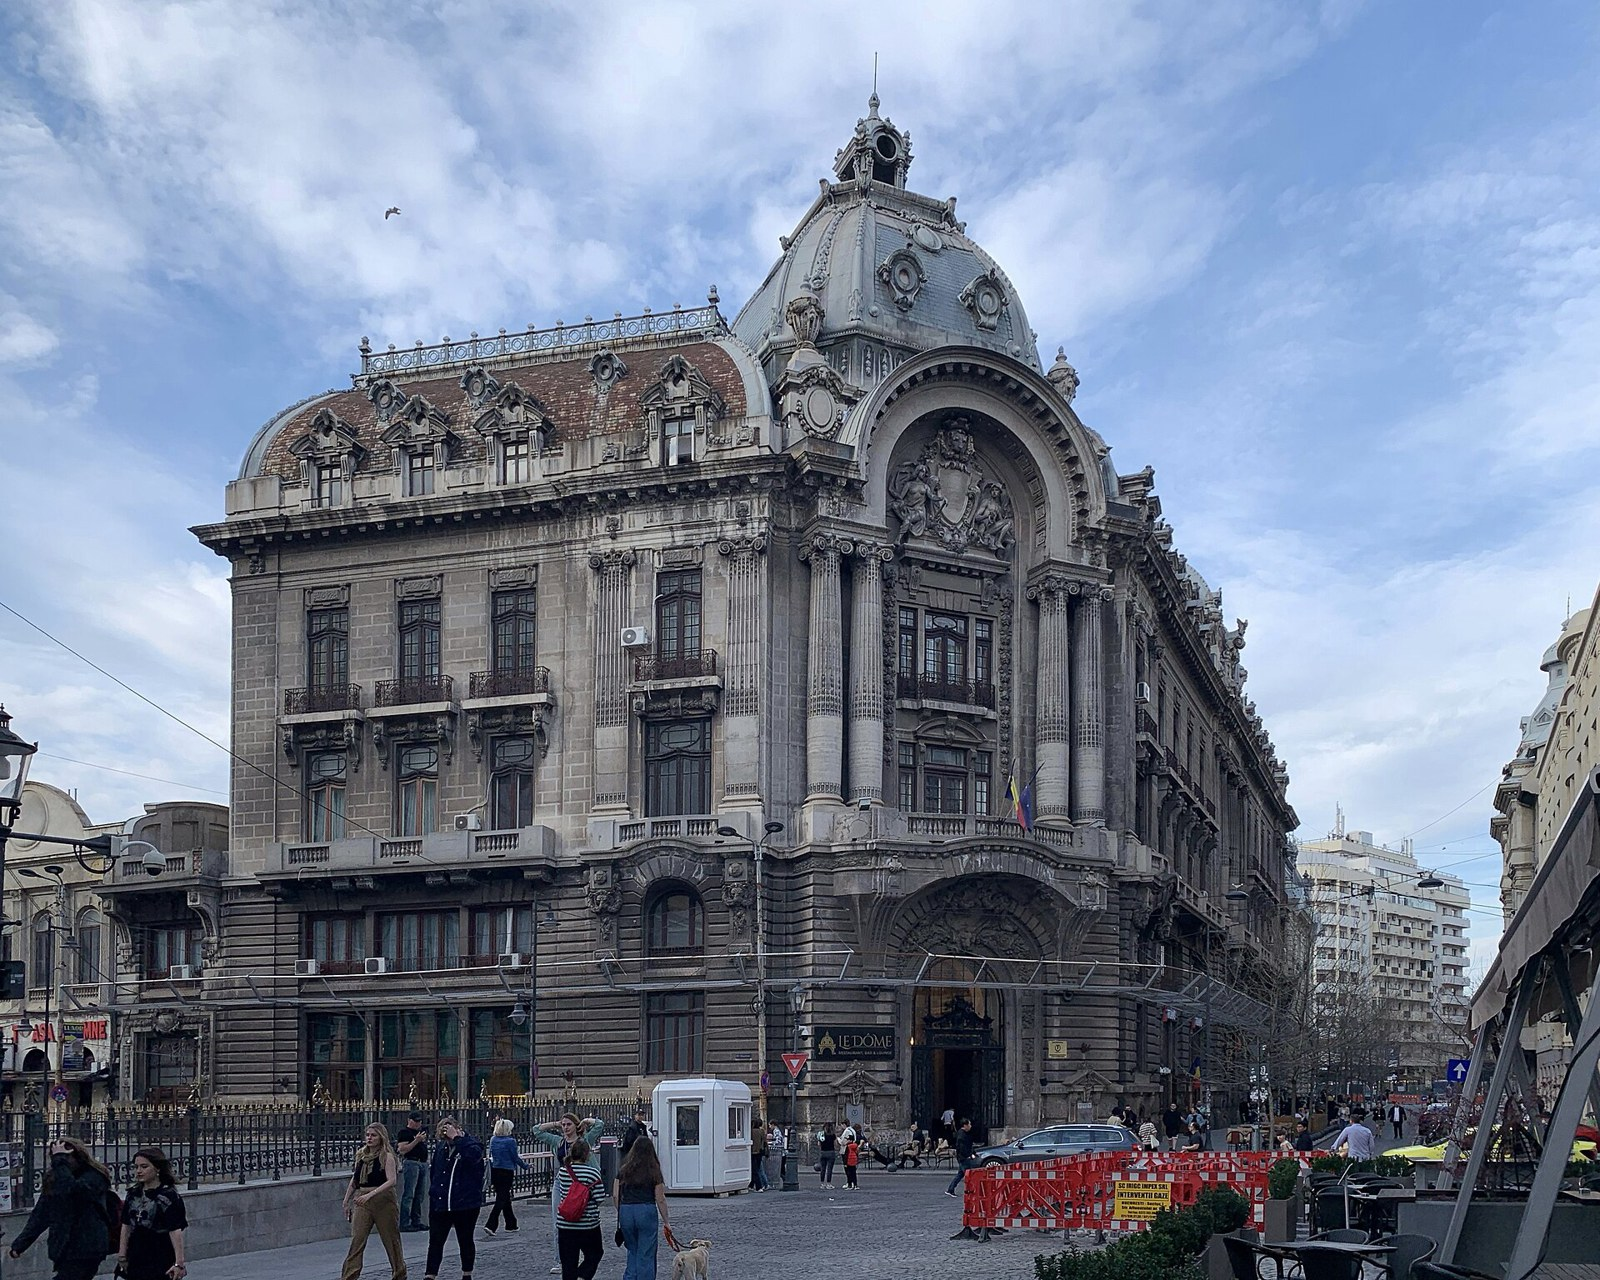
\includegraphics[height=0.40\textheight]{ch0_bvb_palace_2023.jpg}\\[1mm]
\imgcap{Palatul Bursei, București}
\imgcredit{https://commons.wikimedia.org/wiki/File:Bucure\%C8\%99ti_-_Palatul_Bursei_(2023)_-_img_01.jpg}{Foto: Chainwit.\ (2023); CC BY 4.0; Wikimedia Commons}
\end{column}
\end{columns}
\end{frame}

\begin{frame}{Rezultatele învățării}
\itemsize{\small}
\begin{itemize}
    \item Situați fiecare capitol pe drumul de la prețuri la măsurile de risc și numiți întrebarea la care răspunde
    \item Reamintiți formula-cheie, faptul empiric principal și greșeala cea mai frecventă din fiecare capitol
    \item Alegeți testul sau modelul potrivit pentru o întrebare dată despre o serie de randamente
    \item Rezolvați pas cu pas probleme de tip examen și interpretați rezultatul în trei pînă la cinci fraze
    \item Planificați proiectul de echipă, susținerea orală și declararea utilizării AI
\end{itemize}
\end{frame}

\begin{frame}{Bibliografie și instrumente}
\itemsize{\small}
\begin{itemize}
    \item Manual: \refFHH; exerciții rezolvate: \refBHL
    \begin{itemize}
        \item serii de timp și volatilitate: \refTsay; eficiența pieței: \refCLM; măsuri de risc: \refQRM
    \end{itemize}
    \item Quantlet-urile Python ale capitolului: \href{https://github.com/danpele/SFM/tree/main/Quantlets/Ch_16}{Quantlets/Ch\_16}
    \begin{itemize}
        \item cursul într-un singur tabel: S\&P 500, BET și Bitcoin pe aceeași fereastră de timp
    \end{itemize}
    \item Notebook-ul cursului, cursul într-un singur notebook: \href{\colaburl{notebooks/EN/chapter16_lecture_notebook.ipynb}}{deschideți în Google Colab}
    \item Curs video: \quantinar{Statistics of Financial Markets}{https://quantinar.com/course/103/statistics-of-financial-markets}
    \item Autoevaluare: quiz-ul acestui capitol, 20 de întrebări din toate capitolele
\end{itemize}
\end{frame}


%=============================================================================
\section{Harta cursului}
%=============================================================================

\begin{frame}{Harta cursului: \sfmchlinkt{https://danpele.github.io/SFM/RO/Cursuri/capitol0_introducere.pdf}{Capitolele 0}--\sfmchlinkt{https://danpele.github.io/SFM/RO/Cursuri/capitol15_risc_sistemic.pdf}{15}}
\itemsize{\footnotesize}
\begin{center}
\resizebox{0.97\textwidth}{!}{%
\begin{tikzpicture}[
  box/.style={draw=MainBlue, rounded corners=2pt, fill=white, font=\scriptsize, align=center, minimum width=2.2cm, minimum height=0.85cm, text width=2.1cm},
  key/.style={box, draw=IDAred, line width=0.9pt},
  lab/.style={font=\scriptsize\bfseries, text=MainBlue, anchor=east, align=right},
  arr/.style={-{Stealth[length=2mm]}, MainBlue, line width=0.5pt},
  karr/.style={-{Stealth[length=2.4mm]}, IDAred, line width=1.1pt}]
\node[lab] at (-0.1, 0) {Date și\\ distribuții};
\node[box] (c0) at (1.3, 0) {0 Piețe\\ și date};
\node[key] (c1) at (3.8, 0) {1 Randamente,\\ indicatori};
\node[key] (c2) at (6.3, 0) {2 Distribuții,\\ fapte stilizate};
\node[box] (c3) at (8.8, 0) {3 Legi\\ $\alpha$-stabile};
\node[key] (c5) at (11.3, 0) {5 Cozi groase,\\ EVT};
\node[box] (c6) at (13.8, 0) {6 Selecția\\ modelului};
\node[lab] at (-0.1, -1.7) {Timp, volatilitate\\ și risc};
\node[box] (c4) at (1.3, -1.7) {4 Probabilitate,\\ procese};
\node[box] (c7) at (3.8, -1.7) {7 Eficiență,\\ teste VR};
\node[box] (c11) at (6.3, -1.7) {11 Memorie\\ lungă};
\node[box] (c8) at (8.8, -1.7) {8 Estimatori de\\ volatilitate};
\node[key] (c9) at (11.3, -1.7) {9 ARCH, GARCH};
\node[key] (c10) at (13.8, -1.7) {10 VaR, ES,\\ backtesting};
\node[lab] at (-0.1, -3.4) {Aplicații};
\node[box] (c12) at (6.3, -3.4) {12 Modele de\\ scoring};
\node[box] (c13) at (8.8, -3.4) {13 Învățare\\ automată};
\node[box] (c14) at (11.3, -3.4) {14 Active\\ cripto};
\node[box] (c15) at (13.8, -3.4) {15 Risc\\ sistemic};
\draw[arr] (c0) -- (c1); \draw[karr] (c1) -- (c2); \draw[arr] (c2) -- (c3); \draw[arr] (c3) -- (c5); \draw[arr] (c5) -- (c6);
\draw[karr] (c2.south east) -- (c8.north west); \draw[karr] (c5) -- (c10.north west); \draw[arr] (c6) -- (c10);
\draw[arr] (c4) -- (c7); \draw[arr] (c7) -- (c11); \draw[arr] (c11) -- (c8); \draw[karr] (c8) -- (c9); \draw[karr] (c9) -- (c10);
\draw[arr] (c1) -- (c7); \draw[arr] (c4.south) -- (1.3, -2.6) -- (6.3, -2.6) -- (c12.north);
\draw[arr] (c10) -- (c15); \draw[arr] (c10.south west) -- (c14.north east); \draw[arr] (c9.south west) -- (c13.north east);
\end{tikzpicture}}
\end{center}
\vspace{-0.2cm}
\begin{itemize}
    \item Roșu: firul principal, de la randamente și distribuția lor la o măsură de risc pe care o putem testa (\sfmchlink{https://danpele.github.io/SFM/RO/Cursuri/capitol10_var_es_backtesting.pdf}{Capitolul 10})
    \item Rîndul 2: dependența în timp; semnul randamentelor este greu de anticipat (\sfmchlink{https://danpele.github.io/SFM/RO/Cursuri/capitol7_piete_eficiente_mers_aleator_vr.pdf}{Capitolele 7}, \sfmchlink{https://danpele.github.io/SFM/RO/Cursuri/capitol11_piete_fractale_memorie_lunga.pdf}{11}), mărimea lor este previzibilă (\sfmchlink{https://danpele.github.io/SFM/RO/Cursuri/capitol8_estimatori_volatilitate.pdf}{Capitolele 8}--\sfmchlink{https://danpele.github.io/SFM/RO/Cursuri/capitol9_modele_arch_garch.pdf}{9})
    \item Rîndul 3: aceleași instrumente aplicate creditului, predicției, activelor cripto și sistemului bancar
\end{itemize}
\end{frame}

\begin{frame}{Firul principal: de la prețuri la decizii}
\itemsize{\small}
\begin{itemize}
    \item \textbf{Datele} (\sfmchlink{https://danpele.github.io/SFM/RO/Cursuri/capitol0_introducere.pdf}{Capitolele 0}--\sfmchlink{https://danpele.github.io/SFM/RO/Cursuri/capitol1_date_randamente_indicatori.pdf}{1}): prețuri dintr-o singură sursă, ajustate, pe calendarul corect
    \begin{itemize}
        \item randamente: $r_t = \ln(P_t/P_{t-1})$, în \% pe o zi
    \end{itemize}
    \item \textbf{Distribuția} (\sfmchlink{https://danpele.github.io/SFM/RO/Cursuri/capitol2_distributii_clasice_fapte_stilizate.pdf}{Capitolele 2}--\sfmchlink{https://danpele.github.io/SFM/RO/Cursuri/capitol6_selectia_modelului_managementul_riscului.pdf}{6}): cozi groase, nu distribuția Normală
    \begin{itemize}
        \item Student-$t$, legi stabile, EVT; modelul se alege cu verosimilitatea, AIC și teste pentru cozi
    \end{itemize}
    \item \textbf{Dependența în timp} (\sfmchlink{https://danpele.github.io/SFM/RO/Cursuri/capitol7_piete_eficiente_mers_aleator_vr.pdf}{Capitolele 7}--\sfmchlink{https://danpele.github.io/SFM/RO/Cursuri/capitol11_piete_fractale_memorie_lunga.pdf}{11}): semnul este aproape imprevizibil, mărimea este previzibilă
    \begin{itemize}
        \item raportul varianțelor și exponentul Hurst pentru medie; EWMA și GARCH pentru varianță
    \end{itemize}
    \item \textbf{Riscul} (\sfmchlink{https://danpele.github.io/SFM/RO/Cursuri/capitol10_var_es_backtesting.pdf}{Capitolul 10}): VaR 1\% și ES 2,5\%, cu backtesting
    \begin{itemize}
        \item aplicațiile (\sfmchlink{https://danpele.github.io/SFM/RO/Cursuri/capitol12_modele_scoring.pdf}{Capitolele 12}--\sfmchlink{https://danpele.github.io/SFM/RO/Cursuri/capitol15_risc_sistemic.pdf}{15}) refolosesc același lanț: date, distribuție, dependență, risc, evaluare
    \end{itemize}
\end{itemize}
\end{frame}

\begin{frame}{Trei serii, aceeași fereastră: S\&P 500, BET, Bitcoin}
\itemsize{\footnotesize}
\begin{center}
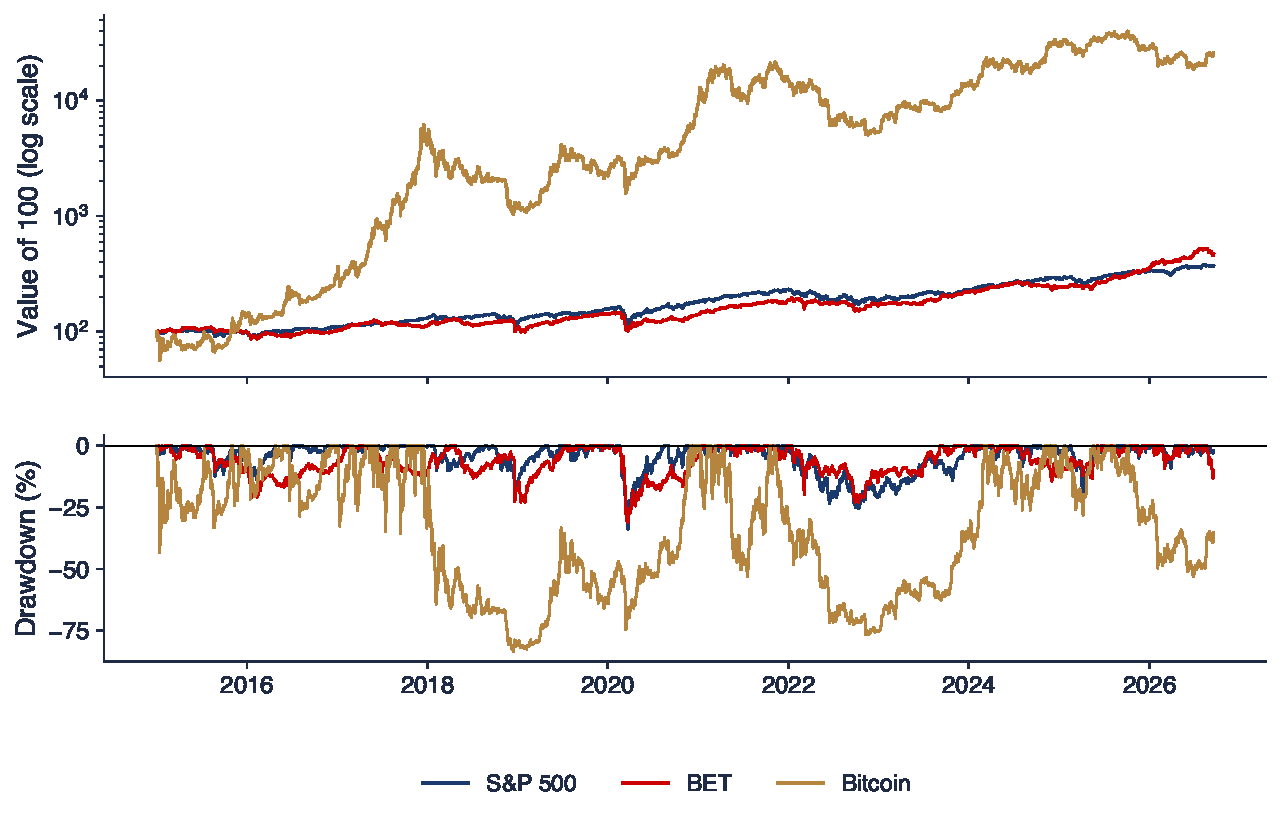
\includegraphics[width=0.97\textwidth,height=0.55\textheight,keepaspectratio]{sfm_ch16_three_series.pdf}
\end{center}
\vspace{-0.25cm}
\begin{itemize}
    \item 100 investiți la 2 ianuarie 2015 (scală logaritmică) și drawdown-ul $P_t/\max_{s \le t}P_s - 1$
    \item Drawdown maxim: S\&P 500 $-33{,}9\%$, BET $-31{,}1\%$ (ambele în martie 2020), Bitcoin $-83{,}4\%$
\end{itemize}
\sfmquantlet{Ch_16}{SFM_ch16_course_summary}
\end{frame}

\begin{frame}{Cursul într-un singur tabel}
\itemsize{\footnotesize}
\begin{center}
\scriptsize
\begin{tabular}{lrrr}
\toprule
\textbf{Randamente logaritmice zilnice} & S\&P 500 & BET & Bitcoin \\
\midrule
Observații (pe an) & 2\,943 (252) & 2\,925 (250) & 4\,278 (365) \\
Randament logaritmic mediu, \% pe an & $11{,}2$ & $13{,}2$ & $47{,}4$ \\
Volatilitate, \% pe an & $17{,}7$ & $15{,}5$ & $66{,}7$ \\
Raportul Sharpe ($r_f = 0$) $\pm$ SE & $0{,}72 \pm 0{,}33$ & $0{,}93 \pm 0{,}35$ & $1{,}04 \pm 0{,}36$ \\
Asimetrie; excesul de boltire & $-0{,}64$; $15{,}8$ & $-1{,}41$; $17{,}8$ & $-0{,}73$; $12{,}2$ \\
Tail index-ul Hill al pierderilor ($k = 2{,}5\%\,n$) & $2{,}75$ & $2{,}19$ & $2{,}67$ \\
Ljung--Box $Q(10)$: $r_t$; $r_t^2$ & $236$; $3166$ & $55$; $701$ & $21$; $211$ \\
VR(5); $Z^*(5)$ robust & $0{,}84$; $-1{,}34$ & $1{,}17$; $1{,}93$ & $0{,}99$; $-0{,}22$ \\
GARCH(1,1)-$t$: $\alpha + \beta$ & $0{,}993$ & $0{,}925$ & $1{,}000$ \\
VaR 1\%: istoric; Normal (\%) & $3{,}29$; $2{,}55$ & $2{,}72$; $2{,}23$ & $10{,}60$; $7{,}99$ \\
ES 2,5\%, istoric (\%) & $3{,}53$ & $3{,}21$ & $10{,}93$ \\
Hurst (R/S): $r_t$; $|r_t|$ & $0{,}53$; $0{,}84$ & $0{,}59$; $0{,}75$ & $0{,}59$; $0{,}78$ \\
\bottomrule
\end{tabular}
\end{center}
\begin{itemize}
    \item Fereastra: 5 ianuarie 2015 -- 18 septembrie 2026; fiecare serie pe calendarul ei (Bitcoin: 365 de zile pe an); valoarea critică $\chi^2(10)$ la 5\%: $18{,}31$
\end{itemize}\sfmquantlet{Ch_16}{SFM_ch16_course_summary}
\end{frame}

\begin{frame}{Interpretarea tabelului}
\itemsize{\small}
\begin{itemize}
    \item \textbf{Randament și risc}: Bitcoin are o volatilitate de circa patru ori mai mare decît a celor doi indici
    \begin{itemize}
        \item rapoartele Sharpe sînt apropiate, dacă ținem seama de erorile lor standard
    \end{itemize}
    \item \textbf{Distribuția}: asimetrie negativă, exces de boltire peste 10, tail index-uri Hill între 2 și 3
    \begin{itemize}
        \item VaR 1\% Normal este prea mic cu 22\% (S\&P 500), 18\% (BET) și 25\% (Bitcoin)
    \end{itemize}
    \item \textbf{Dependența}: statistica Ljung--Box pe $r_t^2$ este de multe ori mai mare decît pe $r_t$
    \begin{itemize}
        \item testul VR robust nu respinge aici mersul aleator la 5\%; $H$ pentru $|r_t|$ este mult peste 0,5
        \item volatilitatea este persistentă: $\alpha + \beta$ aproape de 1 (Bitcoin: un IGARCH, $\alpha + \beta = 1$)
    \end{itemize}
\end{itemize}
\end{frame}

\begin{frame}{Faptele stilizate într-un singur grafic}
\itemsize{\footnotesize}
\begin{center}
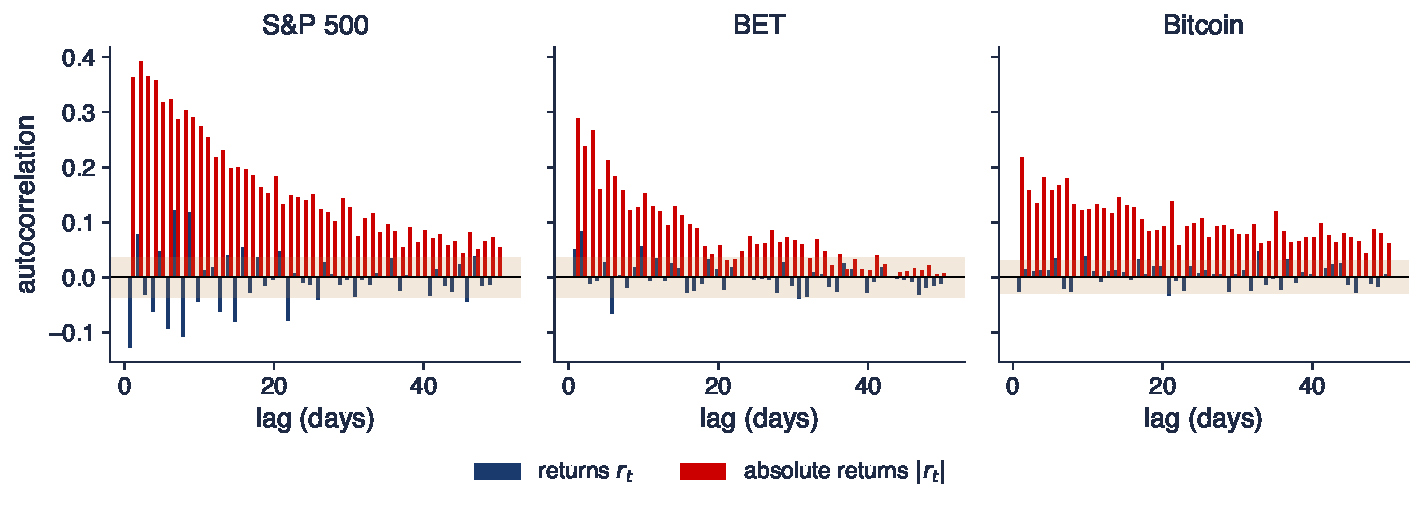
\includegraphics[width=0.97\textwidth,height=0.52\textheight,keepaspectratio]{sfm_ch16_stylised.pdf}
\end{center}
\vspace{-0.25cm}
\begin{itemize}
    \item Randamentele: autocorelații mici și în mare parte în interiorul benzii $\pm 1{,}96/\sqrt{T}$; randamentele absolute: pozitive timp de 50 de zile
    \item Necorelat nu înseamnă independent: $\hat\rho_1(|r|) = 0{,}36$ (S\&P 500), $0{,}29$ (BET), $0{,}22$ (Bitcoin)
\end{itemize}
\sfmquantlet{Ch_16}{SFM_ch16_course_summary}
\end{frame}

\begin{frame}{Recapitulare: harta cursului}
\itemsize{\small}
\begin{itemize}
    \item Un singur lanț în fiecare capitol: date, distribuție, dependență în timp, risc, evaluare
    \item Trei serii străbat cursul: S\&P 500 (o piață dezvoltată), BET (o piață emergentă), Bitcoin (o clasă nouă de active)
    \item Toate trei: cozi groase, randamente aproape necorelate, volatilitate puternic dependentă în timp
\end{itemize}
\end{frame}


%=============================================================================
\section{Capitolele 0--3: date, randamente și distribuții}
%=============================================================================

\begin{frame}{\sfmchlinkt{https://danpele.github.io/SFM/RO/Cursuri/capitol0_introducere.pdf}{Capitolul 0}: introducere (1/2)}
\itemsize{\small}
\begin{itemize}
    \item \textbf{Formule-cheie}
    \begin{itemize}
        \item volatilitatea anualizată $\sigma_{\text{an}} = \sqrt{A}\,\sigma$, $A$ = observații pe an (252 la acțiuni, 365 la cripto)
        \item drawdown $D_t = P_t/\max_{s \le t}P_s - 1$; drawdown maxim MDD $= \min_t D_t$
    \end{itemize}
    \item \textbf{Notațiile}
    \begin{itemize}
        \item $\sigma$: abaterea standard a randamentelor zilnice; $A$: numărul de observații pe an
        \item $P_t$: prețul din ziua $t$; $\max_{s \le t}P_s$: cel mai mare preț pînă în ziua $t$; $D_t \le 0$
    \end{itemize}
\end{itemize}
\end{frame}

\begin{frame}{\sfmchlinkt{https://danpele.github.io/SFM/RO/Cursuri/capitol0_introducere.pdf}{Capitolul 0}: introducere (2/2)}
\itemsize{\small}
\begin{itemize}
    \item \textbf{Fapte empirice}
    \begin{itemize}
        \item din 2015: volatilitate de 17{,}7\% pe an pentru S\&P 500 și de 66{,}7\% pentru Bitcoin
        \item BET: $-82{,}5\%$ între 24 iulie 2007 și 25 februarie 2009; revenire la vîrf abia la 16 martie 2021
    \end{itemize}
    \item \textbf{Greșeli frecvente}
    \begin{itemize}
        \item prețuri din mai multe surse amestecate sau prețuri neajustate pentru acțiuni cu dividende și split-uri
        \item o cifră sau o lucrare de referință obținută cu AI și neverificată
    \end{itemize}
\end{itemize}
\end{frame}

\begin{frame}{\sfmchlinkt{https://danpele.github.io/SFM/RO/Cursuri/capitol1_date_randamente_indicatori.pdf}{Capitolul 1}: date, randamente și indicatori (1/2)}
\itemsize{\small}
\begin{itemize}
    \item \textbf{Formule-cheie}
    \begin{itemize}
        \item $R_t = P_t/P_{t-1} - 1$, $r_t = \ln(1 + R_t)$; randamentele logaritmice se adună în timp, cele simple între active
        \item CAGR $= (P_T/P_0)^{1/Y} - 1$; Sharpe $= (\mu - r_f)/\sigma$, SE $\approx \sqrt{(1 + \mathrm{SR}^2/2)/Y}$; volatility drag $\approx \sigma^2/2$
    \end{itemize}
    \item \textbf{Notațiile}
    \begin{itemize}
        \item $R_t$: randamentul simplu, $r_t$: randamentul logaritmic al perioadei $t$; $P_0$, $P_T$: primul și ultimul preț; $Y$: numărul de ani
        \item $\mu$, $\sigma$: media și volatilitatea anuale; $r_f$: rata fără risc; SR: raportul Sharpe; SE: eroarea lui standard
    \end{itemize}
\end{itemize}
\end{frame}

\begin{frame}{\sfmchlinkt{https://danpele.github.io/SFM/RO/Cursuri/capitol1_date_randamente_indicatori.pdf}{Capitolul 1}: date, randamente și indicatori (2/2)}
\itemsize{\small}
\begin{itemize}
    \item \textbf{Fapte empirice}
    \begin{itemize}
        \item BET din 2015: CAGR 14{,}1\%, volatilitate 15{,}4\%, Sharpe 0{,}93, cu CI 95\% [0{,}36; 1{,}51]
        \item Bitcoin: media aritmetică 69{,}5\% pe an, CAGR doar 60{,}6\%: efectul volatility drag
    \end{itemize}
    \item \textbf{Greșeli frecvente}
    \begin{itemize}
        \item adunarea randamentelor simple în timp; media randamentelor în locul CAGR
        \item anualizarea cu 252 pentru Bitcoin; raportarea raportului Sharpe fără eroarea lui standard
    \end{itemize}
\end{itemize}
\end{frame}

\begin{frame}{\sfmchlinkt{https://danpele.github.io/SFM/RO/Cursuri/capitol2_distributii_clasice_fapte_stilizate.pdf}{Capitolul 2}: distribuții clasice și fapte stilizate (1/2)}
\itemsize{\small}
\begin{itemize}
    \item \textbf{Formule-cheie}
    \begin{itemize}
        \item $S = m_3/m_2^{3/2}$, $K = m_4/m_2^2 - 3$; $\text{JB} = \frac{n}{6}(S^2 + K^2/4) \sim \chi^2(2)$ \refJB
        \item Student-$t(\nu)$: excesul de boltire $6/(\nu - 4)$ pentru $\nu > 4$; Ljung--Box $Q(m) = n(n+2)\sum_h \hat\rho(h)^2/(n - h)$
    \end{itemize}
    \item \textbf{Notațiile}
    \begin{itemize}
        \item $m_k = \frac1n\sum_t (r_t - \bar r)^k$: momentul centrat de ordin $k$; $S$: asimetria; $K$: excesul de boltire (0 pentru distribuția Normală)
        \item JB: Jarque--Bera, $\chi^2(2)$ în ipoteza de normalitate; $\nu$: gradele de libertate; $\hat\rho(h)$: autocorelația la lagul $h$; $m$: numărul de laguri
    \end{itemize}
\end{itemize}
\end{frame}

\begin{frame}{\sfmchlinkt{https://danpele.github.io/SFM/RO/Cursuri/capitol2_distributii_clasice_fapte_stilizate.pdf}{Capitolul 2}: distribuții clasice și fapte stilizate (2/2)}
\itemsize{\small}
\begin{itemize}
    \item \textbf{Fapte empirice}
    \begin{itemize}
        \item BET din 2010: $S = -0{,}98$, $K = 17{,}9$, JB $=$ 56\,762; Student-$t$ estimată: $\hat\nu = 2{,}96$
        \item $\hat\rho_1(r) = 0{,}03$, dar $\hat\rho_1(|r|) = 0{,}34$: cele șase fapte stilizate din \refCont
    \end{itemize}
    \item \textbf{Greșeli frecvente}
    \begin{itemize}
        \item confuzia dintre coeficientul de boltire $K + 3$ și excesul de boltire (distribuția Normală are boltirea 3 și excesul 0)
        \item concluzia de independență trasă dintr-un ACF nesemnificativ al lui $r_t$
    \end{itemize}
\end{itemize}
\end{frame}

\begin{frame}{\sfmchlinkt{https://danpele.github.io/SFM/RO/Cursuri/capitol3_distributii_alfa_stabile.pdf}{Capitolul 3}: distribuții $\alpha$-stabile (1/2)}
\itemsize{\small}
\begin{itemize}
    \item \textbf{Formule-cheie}
    \begin{itemize}
        \item $X_1 + \dots + X_n \overset{d}{=} n^{1/\alpha}X + d_n$; cozi $P(X > x) \sim c\,x^{-\alpha}$; $E|X|^p < \infty$ doar pentru $p < \alpha$
        \item patru parametri: $\alpha$ (cozi), $\beta$ (asimetrie), $\gamma$ (scală), $\delta$ (poziție), în S0 sau S1 \refNolan
    \end{itemize}
    \item \textbf{Notațiile}
    \begin{itemize}
        \item $X_1, \dots, X_n$: copii independente ale lui $X$; $\overset{d}{=}$: aceeași distribuție; $d_n$: o translație; $\alpha \in (0, 2]$: indicele de stabilitate
        \item $c$: o constantă; $p$: ordinul unui moment; S0, S1: două parametrizări ale aceleiași familii
    \end{itemize}
\end{itemize}
\end{frame}

\begin{frame}{\sfmchlinkt{https://danpele.github.io/SFM/RO/Cursuri/capitol3_distributii_alfa_stabile.pdf}{Capitolul 3}: distribuții $\alpha$-stabile (2/2)}
\itemsize{\small}
\begin{itemize}
    \item \textbf{Fapte empirice}
    \begin{itemize}
        \item verosimilitate maximă din 2000: $\hat\alpha = 1{,}49$ (BET), $1{,}54$ (S\&P 500), $1{,}41$ (Bitcoin), ca la bumbacul lui \refMandelbrot
        \item dar varianța de selecție se stabilizează, iar $\hat\alpha$ pentru BET rămîne în jur de 1{,}50 pe date lunare: cozi groase cu varianță finită
    \end{itemize}
    \item \textbf{Greșeli frecvente}
    \begin{itemize}
        \item folosirea abaterii standard ca scală cînd $\alpha < 2$ (varianța nu există)
        \item compararea lui $\delta$ din două programe care folosesc parametrizări diferite
    \end{itemize}
\end{itemize}
\end{frame}

\begin{frame}{Recapitulare: \sfmchlinkt{https://danpele.github.io/SFM/RO/Cursuri/capitol0_introducere.pdf}{capitolele 0}--\sfmchlinkt{https://danpele.github.io/SFM/RO/Cursuri/capitol3_distributii_alfa_stabile.pdf}{3}}
\itemsize{\small}
\begin{itemize}
    \item Întîi date curate și randamente logaritmice; anualizarea se face cu frecvența reală
    \item Randamentele nu sînt Normale: asimetrie negativă, exces de boltire mare, JB respinge peste tot
    \item Legile stabile descriu bine corpul distribuției, dar varianța randamentelor este finită
\end{itemize}
\end{frame}


%=============================================================================
\section{Capitolele 4--7: probabilitate, cozi, alegerea modelului, eficiență}
%=============================================================================

\begin{frame}{\sfmchlinkt{https://danpele.github.io/SFM/RO/Cursuri/capitol4_probabilitate.pdf}{Capitolul 4}: probabilitate (1/2)}
\itemsize{\small}
\begin{itemize}
    \item \textbf{Formule-cheie}
    \begin{itemize}
        \item $\mathrm{Var}(aX + bY) = a^2\sigma_X^2 + b^2\sigma_Y^2 + 2ab\,\mathrm{Cov}(X, Y)$; eroarea Monte Carlo $\sqrt{p(1 - p)/N}$
        \item GBM: $S_t = S_0\exp((\mu - \sigma^2/2)t + \sigma W_t)$, media $S_0e^{\mu t}$, mediana $S_0e^{(\mu - \sigma^2/2)t}$
    \end{itemize}
    \item \textbf{Notațiile}
    \begin{itemize}
        \item $a$, $b$: ponderi; $\sigma_X$, $\sigma_Y$: abateri standard; $p$: probabilitatea estimată; $N$: numărul de extrageri Monte Carlo
        \item GBM (mișcarea browniană geometrică): $S_t$: prețul la momentul $t$ (ani); $\mu$: tendința; $\sigma$: volatilitatea; $W_t \sim N(0, t)$: o mișcare browniană
    \end{itemize}
\end{itemize}
\end{frame}

\begin{frame}{\sfmchlinkt{https://danpele.github.io/SFM/RO/Cursuri/capitol4_probabilitate.pdf}{Capitolul 4}: probabilitate (2/2)}
\itemsize{\small}
\begin{itemize}
    \item \textbf{Fapte empirice}
    \begin{itemize}
        \item S\&P 500 din 2000: o zi sub $-5\%$ are frecvența 0{,}34\%; distribuția Normală dă 0{,}0017\%, de 199 de ori mai puțin
        \item randament mediu 6{,}2\% pe an, cu SE 3{,}7\%: ar fi nevoie de circa 86 de ani de date pentru $t = 3$
    \end{itemize}
    \item \textbf{Greșeli frecvente}
    \begin{itemize}
        \item variabile necorelate considerate independente; media lui $S_t$ confundată cu mediana
        \item o estimare Monte Carlo fără eroarea ei standard
    \end{itemize}
\end{itemize}
\end{frame}

\begin{frame}{\sfmchlinkt{https://danpele.github.io/SFM/RO/Cursuri/capitol5_cozi_groase_evt.pdf}{Capitolul 5}: cozi groase și teoria valorilor extreme (1/2)}
\itemsize{\small}
\begin{itemize}
    \item \textbf{Formule-cheie}
    \begin{itemize}
        \item Hill: $\hat\alpha_k = [\frac1k\sum_{i=1}^k \ln(L_{(i)}/L_{(k+1)})]^{-1}$, SE $\approx \hat\alpha/\sqrt{k}$ \refHill; $\xi = 1/\alpha$
        \item GPD peste $u$: VaR $= u + \frac{\beta}{\xi}[(n\alpha/N_u)^{-\xi} - 1]$; GEV pentru block maxima
    \end{itemize}
    \item \textbf{Notațiile}
    \begin{itemize}
        \item $L_{(i)}$: a $i$-a cea mai mare pierdere; $k$: numărul observațiilor din coadă; $\xi = 1/\alpha$: parametrul de formă al cozii
        \item GPD: $u$: pragul; $\beta$: scala; $N_u$: pierderile peste $u$ din cele $n$; în formula VaR, $\alpha$ este nivelul (1\%), nu tail index-ul
    \end{itemize}
\end{itemize}
\end{frame}

\begin{frame}{\sfmchlinkt{https://danpele.github.io/SFM/RO/Cursuri/capitol5_cozi_groase_evt.pdf}{Capitolul 5}: cozi groase și teoria valorilor extreme (2/2)}
\itemsize{\small}
\begin{itemize}
    \item \textbf{Fapte empirice}
    \begin{itemize}
        \item tail index-ul pierderilor: BET 2{,}57 (CI 95\% [2{,}20; 2{,}95], din 1997), S\&P 500 2{,}97, Bitcoin 2{,}71
        \item BET, VaR 0,1\%: EVT 9{,}6\%, distribuția Normală doar 4{,}5\%
    \end{itemize}
    \item \textbf{Greșeli frecvente}
    \begin{itemize}
        \item alegerea lui $k$ fără graficul Hill; raportarea lui $\hat\alpha$ fără interval
        \item aplicarea estimatorului Hill pe randamente în loc de pierderi $L = -r$
    \end{itemize}
\end{itemize}
\end{frame}

\begin{frame}{\sfmchlinkt{https://danpele.github.io/SFM/RO/Cursuri/capitol6_selectia_modelului_managementul_riscului.pdf}{Capitolul 6}: selecția modelului și managementul riscului (1/2)}
\itemsize{\small}
\begin{itemize}
    \item \textbf{Formule-cheie}
    \begin{itemize}
        \item $LR = 2(\ell_1 - \ell_0) \approx \chi^2(k_1 - k_0)$ pentru modele imbricate; AIC $= -2\ell + 2k$, BIC $= -2\ell + k\ln n$
        \item KS: $D_n = \sup_x|F_n(x) - F(x)|$; Anderson--Darling pune accentul pe cozi
    \end{itemize}
    \item \textbf{Notațiile}
    \begin{itemize}
        \item $\ell_0$, $\ell_1$: log-verosimilitățile maxime ale modelului restrîns și ale celui extins; $k_0$, $k_1$, $k$: numerele de parametri; $n$: volumul eșantionului
        \item $F_n$: funcția de repartiție empirică; $F$: modelul; $D_n$: cea mai mare distanță verticală dintre ele; un AIC sau BIC mai mic este mai bun
    \end{itemize}
\end{itemize}
\end{frame}

\begin{frame}{\sfmchlinkt{https://danpele.github.io/SFM/RO/Cursuri/capitol6_selectia_modelului_managementul_riscului.pdf}{Capitolul 6}: selecția modelului și managementul riscului (2/2)}
\itemsize{\small}
\begin{itemize}
    \item \textbf{Fapte empirice}
    \begin{itemize}
        \item BET din 2000, Anderson--Darling: Normală 161, Student-$t$ 0{,}54, NIG 0{,}40
        \item VaR 1\% pentru BET: distribuția Normală 3{,}19\%, modelele cu cozi groase 3{,}74--4{,}94\%
    \end{itemize}
    \item \textbf{Greșeli frecvente}
    \begin{itemize}
        \item testul LR la frontieră (de exemplu $\nu = \infty$) fără valoarea critică corectată
        \item respingerea tuturor modelelor la $n$ mare, fără ordonarea lor
    \end{itemize}
\end{itemize}
\end{frame}

\begin{frame}{\sfmchlinkt{https://danpele.github.io/SFM/RO/Cursuri/capitol7_piete_eficiente_mers_aleator_vr.pdf}{Capitolul 7}: piețe eficiente, mers aleator și teste VR (1/2)}
\itemsize{\small}
\begin{itemize}
    \item \textbf{Formule-cheie}
    \begin{itemize}
        \item eficiența în formă slabă: prețurile trecute nu prezic randamente în exces \refFama; ipoteza nulă: diferențe de martingal
        \item $\mathrm{VR}(q) = 1 + 2\sum_{k=1}^{q-1}(1 - k/q)\rho(k)$; statistica robustă $Z^*(q) = (\widehat{\mathrm{VR}} - 1)/\sqrt{\hat\theta/T}$ \refLM
    \end{itemize}
    \item \textbf{Notațiile}
    \begin{itemize}
        \item $\rho(k)$: autocorelația la lagul $k$; $q$: orizontul raportului varianțelor; VR $= 1$ pentru un mers aleator
        \item $T$: numărul de randamente; $\hat\theta$: o estimație a varianței robustă la volatility clustering; $Z^* \approx N(0, 1)$ în ipoteza nulă
    \end{itemize}
\end{itemize}
\end{frame}

\begin{frame}{\sfmchlinkt{https://danpele.github.io/SFM/RO/Cursuri/capitol7_piete_eficiente_mers_aleator_vr.pdf}{Capitolul 7}: piețe eficiente, mers aleator și teste VR (2/2)}
\itemsize{\small}
\begin{itemize}
    \item \textbf{Fapte empirice}
    \begin{itemize}
        \item BET din 1997: VR(5) $= 1{,}28$, $Z^* = 5{,}25$ (momentum)
        \item S\&P 500 din 1990: VR(5) $= 0{,}86$, $Z^* = -2{,}76$ (revenire la medie); Bitcoin: $Z^* = -0{,}19$
    \end{itemize}
    \item \textbf{Greșeli frecvente}
    \begin{itemize}
        \item statistica i.i.d.\ $Z(q)$ pe randamente cu volatility clustering (respinge prea des)
        \item rădăcina unitară a prețurilor considerată dovadă de eficiență; predictibilitatea considerată profit
    \end{itemize}
\end{itemize}
\end{frame}

\begin{frame}{Recapitulare: \sfmchlinkt{https://danpele.github.io/SFM/RO/Cursuri/capitol4_probabilitate.pdf}{capitolele 4}--\sfmchlinkt{https://danpele.github.io/SFM/RO/Cursuri/capitol7_piete_eficiente_mers_aleator_vr.pdf}{7}}
\itemsize{\small}
\begin{itemize}
    \item Probabilitățile dau instrumentele: covarianța, varianța condiționată, Monte Carlo cu eroarea lui
    \item Cozile urmează legi de putere cu $\alpha$ între 2 și 4; EVT dă VaR departe în coadă
    \item Modelul se alege după scop și se verifică în afara eșantionului; eficiența se testează cu statistici robuste
\end{itemize}
\end{frame}


%=============================================================================
\section{Capitolele 8--11: volatilitate, risc și memorie}
%=============================================================================

\begin{frame}{\sfmchlinkt{https://danpele.github.io/SFM/RO/Cursuri/capitol8_estimatori_volatilitate.pdf}{Capitolul 8}: estimatori de volatilitate (1/2)}
\itemsize{\small}
\begin{itemize}
    \item \textbf{Formule-cheie}
    \begin{itemize}
        \item EWMA: $\sigma_t^2 = \lambda\sigma_{t-1}^2 + (1 - \lambda)r_{t-1}^2$, timp de înjumătățire $\ln 0{,}5/\ln\lambda$ \refRM
        \item Parkinson: $(\ln H_t - \ln L_t)^2/(4\ln 2)$; ARCH-LM $= nR^2 \sim \chi^2(q)$
    \end{itemize}
    \item \textbf{Notațiile}
    \begin{itemize}
        \item $\lambda \in (0, 1)$: factorul de descompunere; $r_{t-1}$: randamentul de ieri; $H_t$, $L_t$: maximul și minimul zilei $t$
        \item ARCH-LM: $R^2$ al regresiei lui $r_t^2$ pe $q$ laguri ale sale, înmulțit cu $n$; o valoare mare: volatility clustering
    \end{itemize}
\end{itemize}
\end{frame}

\begin{frame}{\sfmchlinkt{https://danpele.github.io/SFM/RO/Cursuri/capitol8_estimatori_volatilitate.pdf}{Capitolul 8}: estimatori de volatilitate (2/2)}
\itemsize{\small}
\begin{itemize}
    \item \textbf{Fapte empirice}
    \begin{itemize}
        \item S\&P 500: Ljung--Box $Q(10)$ este 91 pe $r_t$ și 8015 pe $r_t^2$ (valoarea critică 18{,}31)
        \item EWMA cu $\lambda = 0{,}94$: timp de înjumătățire de 11{,}2 zile; fără ghost effect
    \end{itemize}
    \item \textbf{Greșeli frecvente}
    \begin{itemize}
        \item fereastra mobilă de lungime fixă: o zi extremă intră și iese brusc din calcul (ghost effect)
        \item estimatori de amplitudine pe prețuri cu salturi overnight, fără corecția Yang--Zhang
    \end{itemize}
\end{itemize}
\end{frame}

\begin{frame}{\sfmchlinkt{https://danpele.github.io/SFM/RO/Cursuri/capitol9_modele_arch_garch.pdf}{Capitolul 9}: modele ARCH și GARCH (1/2)}
\itemsize{\small}
\begin{itemize}
    \item \textbf{Formule-cheie}
    \begin{itemize}
        \item GARCH(1,1): $\sigma_t^2 = \omega + \alpha\varepsilon_{t-1}^2 + \beta\sigma_{t-1}^2$, $\bar\sigma^2 = \omega/(1 - \alpha - \beta)$ \refEngle, \refBoll
        \item prognoza $E_t\sigma_{t+h}^2 = \bar\sigma^2 + (\alpha + \beta)^{h-1}(\sigma_{t+1}^2 - \bar\sigma^2)$; timp de înjumătățire $\ln 0{,}5/\ln(\alpha + \beta)$
    \end{itemize}
    \item \textbf{Notațiile}
    \begin{itemize}
        \item $\omega$: constanta; $\alpha$: reacția la șocul de ieri, $\varepsilon_{t-1}$; $\beta$: memoria; $\bar\sigma^2$: varianța pe termen lung
        \item $E_t$: prognoza făcută în ziua $t$; $h$: orizontul, în zile; $\alpha + \beta$: viteza cu care prognoza revine la $\bar\sigma^2$
    \end{itemize}
\end{itemize}
\end{frame}

\begin{frame}{\sfmchlinkt{https://danpele.github.io/SFM/RO/Cursuri/capitol9_modele_arch_garch.pdf}{Capitolul 9}: modele ARCH și GARCH (2/2)}
\itemsize{\small}
\begin{itemize}
    \item \textbf{Fapte empirice}
    \begin{itemize}
        \item GARCH(1,1)-$t$ din 2000: $\alpha + \beta = 0{,}995$ (S\&P 500, timp de înjumătățire 131 de zile), $0{,}991$ (BET, 74 de zile)
        \item Bitcoin: $\alpha + \beta = 1{,}000$, un IGARCH; indicii de acțiuni au nevoie de asimetrie (GJR, EGARCH)
    \end{itemize}
    \item \textbf{Greșeli frecvente}
    \begin{itemize}
        \item inovații Normale pentru randamente cu cozi groase; erori standard nerobuste
        \item raportarea varianței pe termen lung $\omega/(1 - \alpha - \beta)$ cînd $\alpha + \beta \ge 1$
    \end{itemize}
\end{itemize}
\end{frame}

\begin{frame}{\sfmchlinkt{https://danpele.github.io/SFM/RO/Cursuri/capitol10_var_es_backtesting.pdf}{Capitolul 10}: VaR, ES și backtesting (1/2)}
\itemsize{\small}
\begin{itemize}
    \item \textbf{Formule-cheie}
    \begin{itemize}
        \item $\mathrm{VaR}_\alpha = -q_\alpha(X)$, $\mathrm{ES}_\alpha = -\frac1\alpha\int_0^\alpha q_u\,du$; Normal: $-(\mu + \sigma z_\alpha)$, $-\mu + \sigma\varphi(z_\alpha)/\alpha$
        \item Kupiec: $LR_{uc} = -2\ln[(1-\alpha)^{n-x}\alpha^x/((1-\hat\pi)^{n-x}\hat\pi^x)] \sim \chi^2(1)$ \refKupiec; ES este coerent \refArtzner
    \end{itemize}
    \item \textbf{Notațiile}
    \begin{itemize}
        \item $q_\alpha$: cuantila de ordin $\alpha$ a randamentului $X$; $z_\alpha$: cuantila Normală standard; $\varphi$: densitatea Normală standard
        \item $x$: depășirile în $n$ zile; $\hat\pi = x/n$: rata observată; $LR_{uc}$ o compară cu ținta $\alpha$
    \end{itemize}
\end{itemize}
\end{frame}

\begin{frame}{\sfmchlinkt{https://danpele.github.io/SFM/RO/Cursuri/capitol10_var_es_backtesting.pdf}{Capitolul 10}: VaR, ES și backtesting (2/2)}
\itemsize{\small}
\begin{itemize}
    \item \textbf{Fapte empirice}
    \begin{itemize}
        \item S\&P 500, VaR 1\%: istoric 3{,}46\%, Normal 2{,}80\%, adică prea mic cu 19\%
        \item rata depășirilor din 2005: Normal 2{,}71\%, HS 1{,}41\%, GARCH-$t$ 1{,}74\%, FHS 1{,}58\% (ținta 1\%)
    \end{itemize}
    \item \textbf{Greșeli frecvente}
    \begin{itemize}
        \item un VaR negativ sau „VaR 99\%”: în curs scriem VaR 1\%, o pierdere pozitivă
        \item scalarea cu $\sqrt{10}$ ca pentru randamente Normale i.i.d.; verificarea doar a numărului de depășiri, nu și a grupării lor
    \end{itemize}
\end{itemize}
\end{frame}

\begin{frame}{Prognoze VaR 1\% pentru BET: simulare istorică și EWMA-Normal}
\itemsize{\footnotesize}
\begin{center}
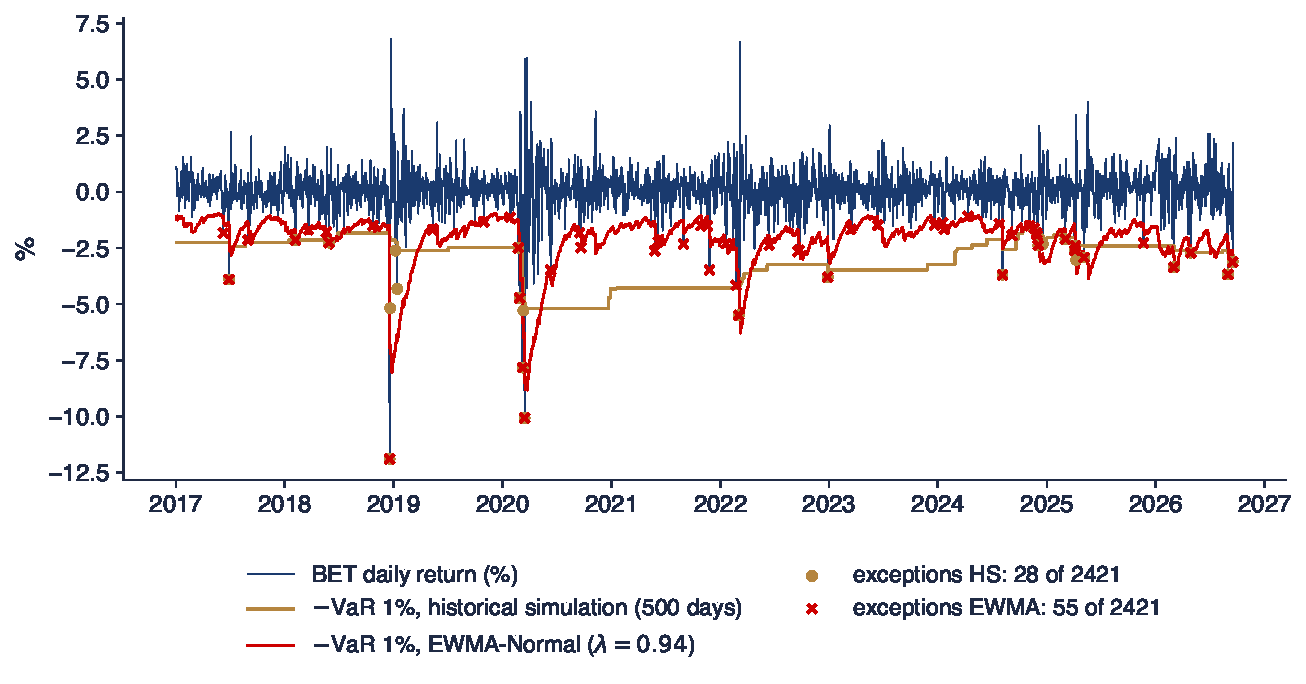
\includegraphics[width=0.97\textwidth,height=0.56\textheight,keepaspectratio]{sfm_ch16_backtest.pdf}
\end{center}
\vspace{-0.25cm}
\begin{itemize}
    \item Din 3 ianuarie 2017, 2\,421 de zile, 24{,}2 depășiri așteptate: HS 28 (1{,}16\%, Kupiec $p = 0{,}450$), EWMA-Normal 55 (2{,}27\%, $p$ $<$\,0{,}001)
    \item EWMA urmărește furtunile, dar cuantila Normală este prea mică; HS are rata corectă, dar depășirile lui vin grupat (cel mult 10 în 250 de zile)
\end{itemize}
\sfmquantlet{Ch_16}{SFM_ch16_course_summary}
\end{frame}

\begin{frame}{\sfmchlinkt{https://danpele.github.io/SFM/RO/Cursuri/capitol11_piete_fractale_memorie_lunga.pdf}{Capitolul 11}: ipoteza piețelor fractale și memoria lungă (1/2)}
\itemsize{\small}
\begin{itemize}
    \item \textbf{Formule-cheie}
    \begin{itemize}
        \item $(R/S)_n \propto n^H$ \refHurst; $H = 0{,}5$: fără memorie, $H > 0{,}5$: persistență; $d = H - 0{,}5$
        \item scalarea riscului: $\mathrm{sd}(r^{(h)}) = h^H\mathrm{sd}(r)$; piețele fractale au nevoie de multe orizonturi investiționale \refPeters
    \end{itemize}
    \item \textbf{Notațiile}
    \begin{itemize}
        \item $(R/S)_n$: amplitudinea rescalată (amplitudinea abaterilor cumulate împărțită la abaterea standard) pe blocuri de $n$ zile
        \item $H$: exponentul Hurst; $d$: parametrul fracționar; $r^{(h)}$: randamentul pe $h$ zile; sd: abaterea standard
    \end{itemize}
\end{itemize}
\end{frame}

\begin{frame}{\sfmchlinkt{https://danpele.github.io/SFM/RO/Cursuri/capitol11_piete_fractale_memorie_lunga.pdf}{Capitolul 11}: ipoteza piețelor fractale și memoria lungă (2/2)}
\itemsize{\small}
\begin{itemize}
    \item \textbf{Fapte empirice}
    \begin{itemize}
        \item BET: $H$ (R/S) $= 0{,}58$ pentru $r_t$, la limita benzii Monte Carlo, iar testul Lo respinge: persistență slabă; $0{,}79$ pentru $|r_t|$
        \item S\&P 500: $0{,}53$ pentru randamente, $0{,}86$ pentru randamente absolute: memoria lungă se află în volatilitate
    \end{itemize}
    \item \textbf{Greșeli frecvente}
    \begin{itemize}
        \item compararea lui $\hat H$ cu 0,5 în locul unei benzi Monte Carlo pentru același $N$ (R/S este deplasat în sus)
        \item rupturi structurale sau efecte GARCH considerate memorie lungă
    \end{itemize}
\end{itemize}
\end{frame}

\begin{frame}{Recapitulare: \sfmchlinkt{https://danpele.github.io/SFM/RO/Cursuri/capitol8_estimatori_volatilitate.pdf}{capitolele 8}--\sfmchlinkt{https://danpele.github.io/SFM/RO/Cursuri/capitol11_piete_fractale_memorie_lunga.pdf}{11}}
\itemsize{\small}
\begin{itemize}
    \item Volatilitatea este latentă, persistentă și previzibilă: EWMA și GARCH o prognozează
    \item O măsură de risc are nevoie atît de o prognoză a volatilității, cît și de o cuantilă cu cozi groase, apoi de backtesting
    \item Memoria lungă: slabă în randamente, puternică în volatilitate
\end{itemize}
\end{frame}


%=============================================================================
\section{Capitolele 12--15: aplicații}
%=============================================================================

\begin{frame}{\sfmchlinkt{https://danpele.github.io/SFM/RO/Cursuri/capitol12_modele_scoring.pdf}{Capitolul 12}: modele de scoring (1/2)}
\itemsize{\small}
\begin{itemize}
    \item \textbf{Formule-cheie}
    \begin{itemize}
        \item EL $=$ PD $\times$ LGD $\times$ EAD; logit $\ln\frac{p}{1-p} = \beta_0 + x^\top\beta$, $e^{\beta_j}$ = raportul șanselor
        \item AUC $= P(s_{\text{rău}} > s_{\text{bun}})$, Gini $= 2\,\mathrm{AUC} - 1$; scorul $Z$ Altman și distanța pînă la nerambursare Merton \refAltman
    \end{itemize}
    \item \textbf{Notațiile}
    \begin{itemize}
        \item EL: pierderea așteptată; PD: probabilitatea de nerambursare; LGD: pierderea în caz de nerambursare; EAD: expunerea la nerambursare
        \item $p$: probabilitatea de nerambursare condiționată de $x$; $\beta_j$: un coeficient; $s$: scorul unui debitor rău sau bun; AUC $= 0{,}5$: nicio discriminare, 1: discriminare perfectă
    \end{itemize}
\end{itemize}
\end{frame}

\begin{frame}{\sfmchlinkt{https://danpele.github.io/SFM/RO/Cursuri/capitol12_modele_scoring.pdf}{Capitolul 12}: modele de scoring (2/2)}
\itemsize{\small}
\begin{itemize}
    \item \textbf{Fapte empirice}
    \begin{itemize}
        \item datele germane de credit (1000 de credite), eșantion de test de 300: AUC $= 0{,}801$, CI 95\% [0{,}75; 0{,}85], Gini 0{,}60
        \item discriminarea nu înseamnă calibrare: le verificăm pe amîndouă, în afara eșantionului
    \end{itemize}
    \item \textbf{Greșeli frecvente}
    \begin{itemize}
        \item acuratețea pe clase dezechilibrate (regula „mereu bun” are deja dreptate în majoritatea cazurilor)
        \item alegerea pragului fără costurile celor două erori
    \end{itemize}
\end{itemize}
\end{frame}

\begin{frame}{\sfmchlinkt{https://danpele.github.io/SFM/RO/Cursuri/capitol13_invatare_automata.pdf}{Capitolul 13}: învățare automată (1/2)}
\itemsize{\small}
\begin{itemize}
    \item \textbf{Formule-cheie}
    \begin{itemize}
        \item deplasare--varianță: $E(y_0 - \hat f)^2 = \text{deplasare}^2 + \mathrm{Var}(\hat f) + \sigma^2$; ridge, lasso, arbori, boosting
        \item în afara eșantionului: $R^2_{OOS} = 1 - \sum(y - \hat y)^2/\sum(y - \tilde y)^2$ față de un reper simplu $\tilde y$ \refGKX
    \end{itemize}
    \item \textbf{Notațiile}
    \begin{itemize}
        \item $y_0$: o observație nouă; $\hat f$: modelul estimat; $\sigma^2$: varianța zgomotului; $\hat y$: prognoza
        \item $\tilde y$: prognoza de referință; sumele parcurg eșantionul de test; $R^2_{OOS} < 0$: mai slab decît reperul
    \end{itemize}
\end{itemize}
\end{frame}

\begin{frame}{\sfmchlinkt{https://danpele.github.io/SFM/RO/Cursuri/capitol13_invatare_automata.pdf}{Capitolul 13}: învățare automată (2/2)}
\itemsize{\small}
\begin{itemize}
    \item \textbf{Fapte empirice}
    \begin{itemize}
        \item semnul randamentelor S\&P 500 din 2008: „mereu creștere” 54{,}4\%, logit 53{,}8\%, boosting 52{,}1\%
        \item volatilitatea realizată: HAR $R^2_{OOS} = 0{,}61$ față de medie; lasso reduce eroarea pătratică a HAR doar cu 7{,}1\%
    \end{itemize}
    \item \textbf{Greșeli frecvente}
    \begin{itemize}
        \item validarea încrucișată aleatoare pe serii de timp (look-ahead bias și leakage)
        \item raportarea celei mai bune dintre multe încercări fără deflatarea raportului Sharpe
    \end{itemize}
\end{itemize}
\end{frame}

\begin{frame}{\sfmchlinkt{https://danpele.github.io/SFM/RO/Cursuri/capitol14_active_cripto.pdf}{Capitolul 14}: active cripto (1/2)}
\itemsize{\small}
\begin{itemize}
    \item \textbf{Formule-cheie}
    \begin{itemize}
        \item anualizăm cu 365 de zile: $\sigma_{\text{an}} = \sqrt{365}\,\sigma$; oferta de Bitcoin limitată la 21 de milioane \refNakamoto
        \item abaterea de la paritate a unui stablecoin $d_t = 10\,000\,(P_t - 1)$ puncte de bază
    \end{itemize}
    \item \textbf{Notațiile}
    \begin{itemize}
        \item $\sigma$: abaterea standard a randamentelor zilnice; activele cripto se tranzacționează 365 de zile pe an
        \item $P_t$: prețul stablecoin-ului în USD; 1 punct de bază $= 0{,}01\%$; $d_t < 0$: sub paritate
    \end{itemize}
\end{itemize}
\end{frame}

\begin{frame}{\sfmchlinkt{https://danpele.github.io/SFM/RO/Cursuri/capitol14_active_cripto.pdf}{Capitolul 14}: active cripto (2/2)}
\itemsize{\small}
\begin{itemize}
    \item \textbf{Fapte empirice}
    \begin{itemize}
        \item Bitcoin: volatilitate de 66{,}6\% pe an cu 365 de zile (55{,}3\% dacă se folosește greșit 252), drawdown maxim $-83{,}4\%$
        \item corelația cu S\&P 500: 0{,}02 înainte de 2020, 0{,}39 după: nu este un activ de refugiu
    \end{itemize}
    \item \textbf{Greșeli frecvente}
    \begin{itemize}
        \item eliminarea weekendurilor din datele cripto sau alinierea randamentelor cripto și de acțiuni pe calendare diferite
        \item un VaR Normal pentru o serie cu $\alpha + \beta = 1$ și tail index sub 3
    \end{itemize}
\end{itemize}
\end{frame}

\begin{frame}{\sfmchlinkt{https://danpele.github.io/SFM/RO/Cursuri/capitol15_risc_sistemic.pdf}{Capitolul 15}: risc sistemic (1/2)}
\itemsize{\small}
\begin{itemize}
    \item \textbf{Formule-cheie}
    \begin{itemize}
        \item CoVaR: VaR-ul sistemului cînd o instituție se află la VaR-ul ei; $\Delta\mathrm{CoVaR} = b\,(q_{50} - q_\alpha)$ dintr-o regresie cuantilică \refAB
        \item MES, SRISK, rețele Granger și tabelul de conectivitate Diebold--Yilmaz \refDY
    \end{itemize}
    \item \textbf{Notațiile}
    \begin{itemize}
        \item $b$: panta regresiei cuantilice a sistemului pe bancă; $q_\alpha$, $q_{50}$: cuantila de ordin $\alpha$ și mediana randamentului băncii
        \item MES: pierderea medie a băncii în cele mai proaste zile ale pieței; SRISK: capitalul lipsă într-o criză
    \end{itemize}
\end{itemize}
\end{frame}

\begin{frame}{\sfmchlinkt{https://danpele.github.io/SFM/RO/Cursuri/capitol15_risc_sistemic.pdf}{Capitolul 15}: risc sistemic (2/2)}
\itemsize{\small}
\begin{itemize}
    \item \textbf{Fapte empirice}
    \begin{itemize}
        \item Banca Transilvania și BET: VaR 1\% 5{,}23\%, $\Delta$CoVaR 1\% 3{,}31 pp (CI 95\% [2{,}35; 4{,}78])
        \item 11 bănci americane și europene: conectivitate totală de circa 78\%
    \end{itemize}
    \item \textbf{Greșeli frecvente}
    \begin{itemize}
        \item ordonarea băncilor după propriul VaR: un VaR mare nu înseamnă neapărat o contribuție mare la riscul sistemului
        \item corelații comparate între perioade calme și de criză fără ajustarea Forbes--Rigobon
    \end{itemize}
\end{itemize}
\end{frame}

\begin{frame}{Recapitulare: \sfmchlinkt{https://danpele.github.io/SFM/RO/Cursuri/capitol12_modele_scoring.pdf}{capitolele 12}--\sfmchlinkt{https://danpele.github.io/SFM/RO/Cursuri/capitol15_risc_sistemic.pdf}{15}}
\itemsize{\small}
\begin{itemize}
    \item Scoring: discriminare (AUC, Gini) și calibrare, în afara eșantionului, cu costuri
    \item Machine learning: evaluat față de un reper simplu, cu validare walk-forward
    \item Cripto și risc sistemic: aceleași instrumente, cu calendarul corect și măsuri condiționate ale cozii
\end{itemize}
\end{frame}


%=============================================================================
\section{Trusa de instrumente}
%=============================================================================

\begin{frame}{Trusa de instrumente (1/2): randamente, distribuții și cozi}
\itemsize{\small}
\begin{center}
\footnotesize
\begin{tabular}{>{\raggedright\arraybackslash}p{3.6cm}>{\raggedright\arraybackslash}p{3.4cm}>{\raggedright\arraybackslash}p{3.4cm}c}
\toprule
\textbf{Întrebarea} & \textbf{Instrumentul} & \textbf{Decizia} & \textbf{Cap.} \\
\midrule
Cît de bună a fost investiția? & CAGR, Sharpe, Sortino, MDD & comparăm cu SE și un reper & 1 \\
Sînt randamentele Normale? & JB, QQ plot & respingem dacă JB $> 5{,}99$ & 2 \\
Cît de groase sînt cozile? & graficul Hill, GPD, $\alpha$ stabil & momentele există pentru $p < \alpha$ & 3, 5 \\
Ce distribuție se potrivește? & LR, AIC, BIC, KS, AD & AIC minim; AD pentru cozi & 6 \\
Cît de rară este o pierdere de $x$? & funcția de repartiție empirică, EVT, Monte Carlo & raportăm SE a estimării & 4, 5 \\
Este varianța finită? & varianța cumulativă, agregarea lui $\hat\alpha$ & varianță de selecție stabilă: finită & 3 \\
\bottomrule
\end{tabular}
\end{center}
\end{frame}

\begin{frame}{Trusa de instrumente (2/2): dependență în timp, volatilitate și risc}
\itemsize{\small}
\begin{center}
\footnotesize
\begin{tabular}{>{\raggedright\arraybackslash}p{3.6cm}>{\raggedright\arraybackslash}p{3.4cm}>{\raggedright\arraybackslash}p{3.4cm}c}
\toprule
\textbf{Întrebarea} & \textbf{Instrumentul} & \textbf{Decizia} & \textbf{Cap.} \\
\midrule
Sînt randamentele previzibile? & ACF, Ljung--Box, VR robust $Z^*(q)$ & respingem dacă $|Z^*| > 1{,}96$ & 7 \\
Există volatility clustering? & Ljung--Box pe $r_t^2$, ARCH-LM & respingem: modelăm varianța & 8 \\
Cît de volatil va fi mîine? & EWMA, GARCH(1,1)-$t$, GJR & QLIKE față de un reper & 8, 9 \\
Cît putem pierde? & VaR 1\%, ES 2,5\%: HS, $t$, EVT, FHS & Kupiec, Christoffersen, semaforul Basel & 10 \\
Există memorie lungă? & R/S, DFA, GPH, testul Lo & comparăm cu o bandă Monte Carlo & 11 \\
Cine va intra în nerambursare? & logit, LDA, AUC, Gini & în afara eșantionului, cu costuri & 12 \\
Ce bancă contează pentru sistem? & CoVaR, MES, SRISK & CI bootstrap pentru $\Delta$CoVaR & 15 \\
\bottomrule
\end{tabular}
\end{center}
\end{frame}

\begin{frame}{Convențiile folosite în tot cursul}
\itemsize{\small}
\begin{itemize}
    \item \textbf{Randamentele}: randamente logaritmice zilnice în \%, $r_t = 100\,(\ln P_t - \ln P_{t-1})$
    \begin{itemize}
        \item portofolii: randamente simple, după alinierea prețurilor pe zilele comune
    \end{itemize}
    \item \textbf{Anualizarea}: media $\times A$, volatilitatea $\times\sqrt{A}$, cu $A$ real
    \begin{itemize}
        \item $A$: numărul de observații pe an: circa 252 pentru acțiuni și indici, 365 pentru cripto
    \end{itemize}
    \item \textbf{Riscul}: nivelul este probabilitatea cozii: VaR 1\%, ES 2,5\%
    \begin{itemize}
        \item $\mathrm{VaR}_\alpha = -q_\alpha > 0$, o pierdere; simularea istorică cu $k = \lceil n\alpha \rceil$
    \end{itemize}
    \item \textbf{Testele}: precizăm $H_0$, statistica, distribuția ei, valoarea critică și decizia la 5\%
    \begin{itemize}
        \item apoi o frază despre semnificația deciziei pentru date
    \end{itemize}
\end{itemize}
\end{frame}

\begin{frame}{Șase capcane din tot cursul}
\itemsize{\small}
\begin{itemize}
    \item \textbf{Datele}: alinierea randamentelor în loc de prețuri; prețuri neajustate; weekenduri eliminate la cripto
    \item \textbf{Distribuția}: distribuția Normală pentru cuantilele din coadă; confuzia dintre boltire și excesul de boltire
    \item \textbf{Inferența}: erori standard i.i.d.\ în prezența volatility clustering; o statistică fără SE
    \item \textbf{Timpul}: look-ahead bias, parametri estimați pe tot eșantionul și folosiți în trecut
    \item \textbf{Riscul}: semnul și nivelul VaR; ES comparat cu VaR la niveluri diferite
    \item \textbf{Interpretarea}: semnificația statistică luată drept importanță economică, predictibilitatea drept profit
\end{itemize}
\end{frame}


%=============================================================================
\section{Examenul}
%=============================================================================

\begin{frame}{Examenul scris: formatul}
\itemsize{\small}
\begin{columns}[T]
\begin{column}{0.58\textwidth}
\begin{itemize}
    \item \textbf{70\% din nota finală}; scris, 2 ore; calculatorul este permis
    \begin{itemize}
        \item toate subiectele sînt obligatorii; 9 puncte plus 1 punct din oficiu
    \end{itemize}
    \item \textbf{Valorile utile sînt date} pe subiect
    \begin{itemize}
        \item cuantile ale distribuției Normale și Student-$t$, valori critice $\chi^2$, logaritmi și radicali
    \end{itemize}
    \item \textbf{Fiecare subiect}: un context scurt, cifre, un tabel sau un grafic, una sau două cerințe
    \begin{itemize}
        \item un calcul urmat de o interpretare în trei pînă la cinci fraze
    \end{itemize}
\end{itemize}
\end{column}
\begin{column}{0.38\textwidth}
\centering
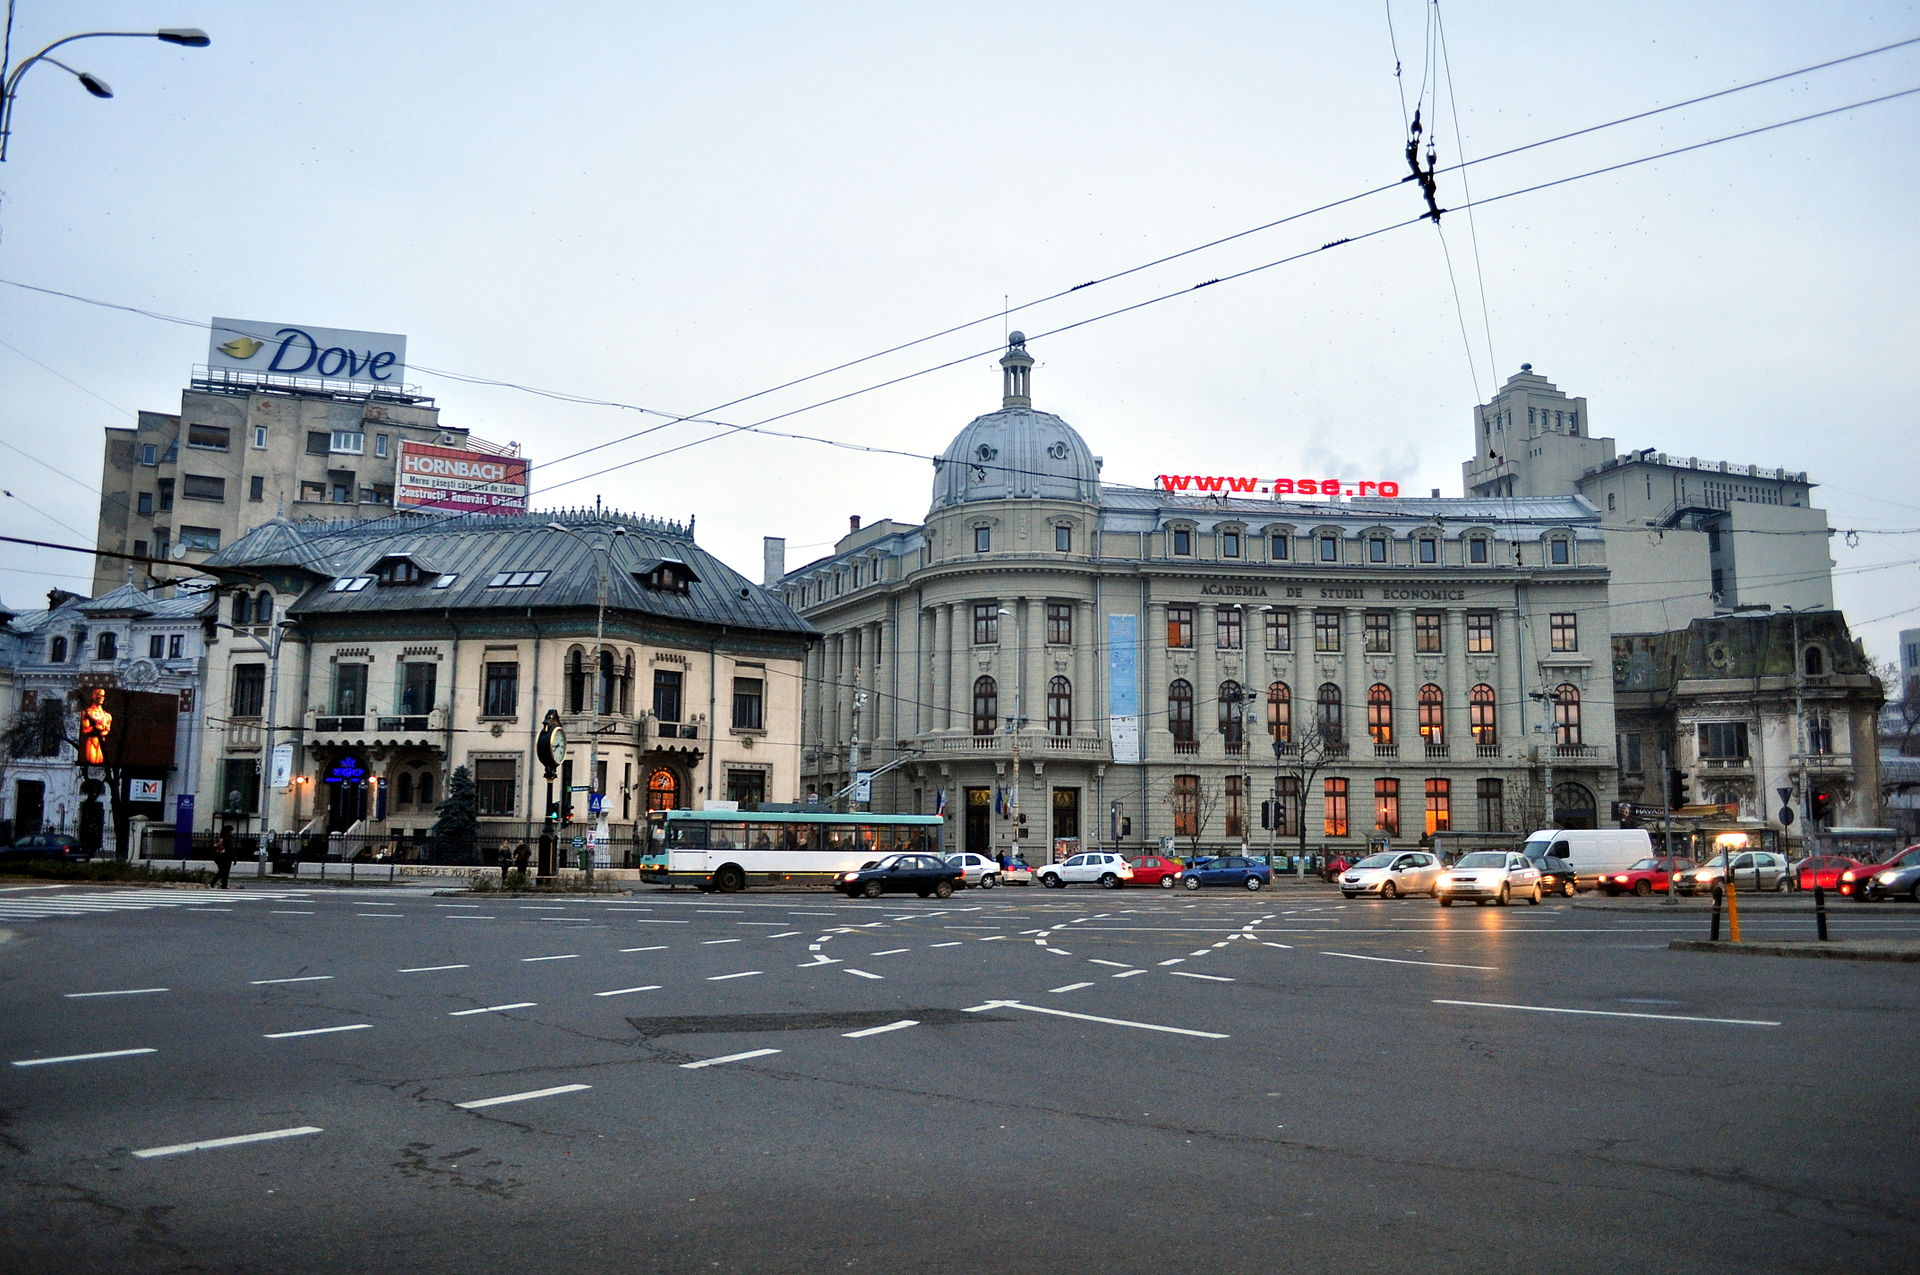
\includegraphics[height=0.40\textheight]{ch0_ase_2014.jpg}\\[1mm]
\imgcap{Academia de Studii Economice din București}
\imgcredit{https://commons.wikimedia.org/wiki/File:Bucharest_-_Academie_de_Studii_Economice_01.jpg}{Foto: Joe Mabel (2014); CC BY 3.0; Wikimedia Commons}
\end{column}
\end{columns}
\end{frame}

\begin{frame}{Conținutul evaluat}
\itemsize{\small}
\begin{itemize}
    \item \textbf{\sfmchlink{https://danpele.github.io/SFM/RO/Cursuri/capitol0_introducere.pdf}{Capitolele 0}--\sfmchlink{https://danpele.github.io/SFM/RO/Cursuri/capitol15_risc_sistemic.pdf}{15}}: cursuri și seminarii
    \begin{itemize}
        \item definițiile și formulele de pe slide-urile „Noțiuni necesare azi” ale fiecărui seminar
        \item calculele din Partea A a seminariilor, pe hîrtie
    \end{itemize}
    \item \textbf{Interpretarea rezultatelor obținute cu software}
    \begin{itemize}
        \item tabele și grafice ca în Partea B: estimări, statistici de test, p-value-uri, backtesting
        \item la examen nu se scrie cod
    \end{itemize}
    \item \textbf{Înțelegere, nu memorare}
    \begin{itemize}
        \item de ce o metodă dă greș pe randamentele financiare, ce test răspunde la ce întrebare
    \end{itemize}
\end{itemize}
\end{frame}

\begin{frame}{Criterii de notare}
\itemsize{\small}
\begin{itemize}
    \item \textbf{Metoda}: formula, cu cifrele înlocuite
    \begin{itemize}
        \item o metodă corectă cu o greșeală de calcul primește cea mai mare parte a punctajului
    \end{itemize}
    \item \textbf{Rezultatul}: cifra, cu unitatea de măsură (\%, zile, lei) și semnul ei
    \begin{itemize}
        \item pentru un test: $H_0$, statistica, valoarea critică sau p-value-ul, decizia
    \end{itemize}
    \item \textbf{Interpretarea}: trei pînă la cinci fraze, statistice și economice
    \begin{itemize}
        \item precizați ipotezele unei formule aproximative (i.i.d., distribuția Normală, $n$ mare)
        \item o cifră corectă cu o interpretare greșită nu primește tot punctajul
    \end{itemize}
\end{itemize}
\end{frame}

\begin{frame}{Tipuri de probleme}
\itemsize{\small}
\begin{center}
\footnotesize
\begin{tabular}{>{\raggedright\arraybackslash}p{4.2cm}>{\raggedright\arraybackslash}p{1.4cm}>{\raggedright\arraybackslash}p{5.3cm}}
\toprule
\textbf{Tipul} & \textbf{Capitole} & \textbf{Exemplu în acest capitol} \\
\midrule
randamente, anualizare, performanță & 0, 1 & Problema 1: CAGR, drawdown, volatility drag \\
momente, normalitate, cozi & 2, 3, 5, 6 & Problema 2: JB, Student-$t$, Hill \\
probabilitate și simulare & 4 & Problema 3: portofoliu, Monte Carlo, GBM \\
eficiență și memorie & 7, 11 & Problemele 4 și 7: Ljung--Box, VR, Hurst \\
volatilitate & 8, 9, 14 & Problema 5: GARCH, EWMA, anualizarea Bitcoin \\
măsuri de risc și backtesting & 10 & Problema 6: VaR, ES, Kupiec, semaforul Basel \\
risc de credit și risc sistemic & 12, 13, 15 & Problema 8: matricea de confuzie, EL, $\Delta$CoVaR \\
\bottomrule
\end{tabular}
\end{center}
\begin{itemize}
    \item Cele opt probleme de mai jos sînt exemple de recapitulare, cu rezolvări complete; examenul are subiecte proprii
\end{itemize}
\end{frame}

\begin{frame}{Problema 1: randamente și drawdown}
\itemsize{\footnotesize}
\begin{itemize}
    \item \textbf{Context}
    \begin{itemize}
        \item Un indice valorează 100, 160, 64 și 96 la sfîrșitul anilor 0, 1, 2 și 3
    \end{itemize}
    \item \textbf{Cerințe}
\begin{enumerate}
    \item Calculați randamentele simple $R_t$ și randamentele logaritmice $r_t$ ale celor trei ani.
    \item Calculați randamentul total în două moduri: din $\sum_t r_t$ și din prețuri.
    \item Calculați media aritmetică a lui $R_t$ și CAGR, apoi explicați diferența.
    \item Calculați drawdown-ul maxim și cîștigul necesar de la minim pînă la vîrful anterior.
\end{enumerate}
\end{itemize}
\end{frame}

\begin{frame}{Problema 1: rezolvare}
\itemsize{\footnotesize}
\begin{enumerate}
    \item $R = 60\%; -60\%; 50\%$; $r = \ln 1{,}6 = 0{,}470$, $\ln 0{,}4 = -0{,}916$, $\ln 1{,}5 = 0{,}405$
    \item $\sum_t r_t = -0{,}041 = \ln(96/100)$, deci randamentul total este $e^{-0{,}041} - 1 = -4\%$, la fel ca $96/100 - 1$
    \item media aritmetică $(60 - 60 + 50)/3 = 16{,}67\%$; CAGR $= (96/100)^{1/3} - 1 = -1{,}35\%$
    \item MDD $= 64/160 - 1 = -60\%$; pentru revenirea de la 64 la 160, indicele are nevoie de $160/64 - 1 = 150\%$
\end{enumerate}
\begin{itemize}
    \item \textbf{Interpretare}
    \begin{itemize}
        \item Un randament mediu pozitiv și totuși o pierdere de bani: volatilitatea reduce creșterea compusă (volatility drag)
        \item Randamentele logaritmice se adună în timp; cele simple nu
    \end{itemize}
\end{itemize}
\end{frame}

\begin{frame}{Problema 2: distribuție și cozi}
\itemsize{\footnotesize}
\begin{itemize}
    \item \textbf{Context}
    \begin{itemize}
        \item $n = 1000$ de randamente zilnice cu asimetria $S = -0{,}5$ și excesul de boltire $K = 6$
        \item Cele mai mari cinci pierderi, în \%: $8{,}2$; $6{,}5$; $5{,}9$; $5{,}1$; $4{,}6$; $\chi^2_{0,95}(2) = 5{,}99$
    \end{itemize}
    \item \textbf{Cerințe}
\begin{enumerate}
    \item Calculați statistica Jarque--Bera și cele două componente ale ei, apoi decideți la 5\%.
    \item Determinați numărul de grade de libertate $\nu$ al unei distribuții Student-$t$ cu același exces de boltire.
    \item Calculați estimarea Hill $\hat\alpha$ cu $k = 4$.
    \item Precizați ce momente ale pierderilor există dacă $\alpha = \hat\alpha$ și dacă o lege stabilă cu $\alpha < 2$ este compatibilă cu acest rezultat.
\end{enumerate}
\end{itemize}
\end{frame}

\begin{frame}{Problema 2: rezolvare}
\itemsize{\footnotesize}
\begin{enumerate}
    \item componenta asimetriei $\frac{1000}{6}(0{,}25) = 41{,}67$; componenta boltirii $\frac{1000}{24}(36) = 1500{,}0$; JB $= 1541{,}7 > 5{,}99$: normalitatea se respinge
    \item $6/(\nu - 4) = 6 \Rightarrow \nu = 5$
    \item $\ln(8{,}2/4{,}6) = 0{,}578$, $\ln(6{,}5/4{,}6) = 0{,}346$, $\ln(5{,}9/4{,}6) = 0{,}249$, $\ln(5{,}1/4{,}6) = 0{,}103$; media $0{,}3190$, deci $\hat\alpha = 3{,}14$
    \item există momentele de ordin $p < 3{,}14$: media, varianța, asimetria; boltirea nu există; o lege stabilă cu $\alpha < 2$ (varianță infinită) are cozi mai groase decît aceste date
\end{enumerate}
\begin{itemize}
    \item \textbf{Interpretare}
    \begin{itemize}
        \item Componenta boltirii domină JB: cozile groase, nu asimetria, duc la respingerea normalității
        \item $k = 4$ dă o estimare foarte zgomotoasă a lui $\hat\alpha$ (SE $\approx \hat\alpha/2$); în practică, $k$ se alege din graficul Hill
    \end{itemize}
\end{itemize}
\end{frame}

\begin{frame}{Problema 3: portofoliu, Monte Carlo și GBM}
\itemsize{\footnotesize}
\begin{itemize}
    \item \textbf{Context}
    \begin{itemize}
        \item Două active: volatilități zilnice de $1{,}5\%$ și $2{,}5\%$, corelație $0{,}3$, ponderi 60\% și 40\%
        \item Prețul unei acțiuni urmează un GBM cu $\mu = 8\%$, $\sigma = 25\%$ pe an, $S_0 = 100$
    \end{itemize}
    \item \textbf{Cerințe}
\begin{enumerate}
    \item Calculați volatilitatea zilnică a portofoliului și comparați-o cu media ponderată a volatilităților.
    \item Un studiu Monte Carlo cu $N = 10\,000$ de extrageri estimează o probabilitate de 1\%; calculați SE și un interval de 95\%.
    \item Calculați media și mediana lui $S_1$, precum și $P(S_1 < S_0)$.
\end{enumerate}
\end{itemize}
\end{frame}

\begin{frame}{Problema 3: rezolvare}
\itemsize{\footnotesize}
\begin{enumerate}
    \item $\sigma_p^2 = 0{,}81 + 1{,}00 + 0{,}54 = 2{,}35$, $\sigma_p = 1{,}53\%$, sub media ponderată $1{,}90\%$
    \item SE $= \sqrt{0{,}01 \times 0{,}99/10\,000} = 0{,}099\%$; interval $[0{,}80\%; 1{,}20\%]$
    \item media $100e^{0{,}08} = 108{,}33$; mediana $100e^{0{,}08 - 0{,}03125} = 105{,}00$; $P(S_1 < S_0) = \Phi(-0{,}0488/0{,}25) = \Phi(-0{,}195) = 42{,}3\%$
\end{enumerate}
\begin{itemize}
    \item \textbf{Interpretare}
    \begin{itemize}
        \item Diversificarea: cu $\rho < 1$, portofoliul este mai puțin riscant decît media componentelor
        \item Un investitor într-un GBM pierde bani după un an cu probabilitatea de 42{,}3\%, deși prețul așteptat crește
    \end{itemize}
\end{itemize}
\end{frame}

\begin{frame}{Problema 4: autocorelație și raportul varianțelor}
\itemsize{\footnotesize}
\begin{itemize}
    \item \textbf{Context}
    \begin{itemize}
        \item $T = 2500$ de randamente zilnice; $\hat\rho(1) = 0{,}06$, $\hat\rho(2) = 0{,}02$, $\hat\rho(3) = -0{,}01$, $\hat\rho(4) = 0{,}01$; $\chi^2_{0,95}(4) = 9{,}49$
        \item Eroarea standard robustă la heteroscedasticitate a lui $\widehat{\mathrm{VR}}(5)$ este $0{,}065$
    \end{itemize}
    \item \textbf{Cerințe}
\begin{enumerate}
    \item Calculați statistica Ljung--Box $Q(4)$ și decideți la 5\%.
    \item Calculați $\mathrm{VR}(5) = 1 + 2\sum_{k=1}^{4}(1 - k/5)\hat\rho(k)$.
    \item Calculați statistica i.i.d.\ $Z(5)$, cu SE $= \sqrt{2(2q-1)(q-1)/(3qT)}$, și statistica robustă $Z^*(5)$, apoi decideți la 5\%.
\end{enumerate}
\end{itemize}
\end{frame}

\begin{frame}{Problema 4: rezolvare}
\itemsize{\footnotesize}
\begin{enumerate}
    \item $Q(4) = T(T+2)\sum_{k=1}^{4}\hat\rho_k^2/(T-k) = 10{,}51$, apropiat de $T\sum_k\hat\rho_k^2$, cu $\sum_k\hat\rho_k^2 = 0{,}0042$; $10{,}51 > 9{,}49$: se respinge absența autocorelației
    \item $\mathrm{VR}(5) = 1 + 2(0{,}8 \times 0{,}06 + 0{,}6 \times 0{,}02 - 0{,}4 \times 0{,}01 + 0{,}2 \times 0{,}01) = 1 + 2 \times 0{,}058 = 1{,}116$
    \item SE $= \sqrt{72/37\,500} = 0{,}0438$, $Z(5) = 2{,}65 > 1{,}96$; $Z^*(5) = (1{,}116 - 1)/0{,}065 = 1{,}78 < 1{,}96$ (robust)
\end{enumerate}
\begin{itemize}
    \item \textbf{Interpretare}
    \begin{itemize}
        \item VR $> 1$: autocorelație pozitivă (momentum); testul i.i.d.\ respinge mersul aleator
        \item Testul robust nu îl respinge: volatility clustering mărește artificial statistica $Z(5)$; decizia care se raportează este cea robustă
    \end{itemize}
\end{itemize}
\end{frame}

\begin{frame}{Problema 5: prognoze de volatilitate}
\itemsize{\footnotesize}
\begin{itemize}
    \item \textbf{Context}
    \begin{itemize}
        \item GARCH(1,1) pentru randamente zilnice în \%: $\omega = 0{,}03$, $\alpha = 0{,}09$, $\beta = 0{,}89$; azi $\sigma_t^2 = 1{,}8$ și $\varepsilon_t = -2{,}5$
        \item Bitcoin: abaterea standard zilnică $3{,}5\%$
    \end{itemize}
    \item \textbf{Cerințe}
\begin{enumerate}
    \item Calculați $\sigma_{t+1}^2$ și VaR 1\% Normal pe o zi (medie zero, $z_{0,01} = -2{,}326$).
    \item Calculați persistența, timpul de înjumătățire, varianța pe termen lung și volatilitatea anuală pe termen lung.
    \item Calculați $E_t[\sigma_{t+10}^2]$ și prognoza EWMA cu $\lambda = 0{,}94$.
    \item Anualizați volatilitatea Bitcoin.
\end{enumerate}
\end{itemize}
\end{frame}

\begin{frame}{Problema 5: rezolvare}
\itemsize{\footnotesize}
\begin{enumerate}
    \item $\sigma_{t+1}^2 = 0{,}03 + 0{,}5625 + 1{,}602 = 2{,}1945$, $\sigma_{t+1} = 1{,}481\%$; VaR 1\% $= 2{,}326 \times 1{,}481 = 3{,}45\%$
    \item $\alpha + \beta = 0{,}98$; $h_{1/2} = \ln 0{,}5/\ln 0{,}98 = 34{,}3$ zile; $\bar\sigma^2 = 0{,}03/0{,}02 = 1{,}50$; $\sqrt{252 \times 1{,}50} = 19{,}44\%$ pe an
    \item $E_t\sigma_{t+10}^2 = 1{,}50 + 0{,}98^9(2{,}1945 - 1{,}50) = 2{,}079$; EWMA: $0{,}94 \times 1{,}8 + 0{,}06 \times 6{,}25 = 2{,}067$
    \item Bitcoin se tranzacționează în fiecare zi: $3{,}5 \times \sqrt{365} = 66{,}9\%$; cu 252, rezultatul ar fi greșit: $55{,}6\%$
\end{enumerate}
\begin{itemize}
    \item \textbf{Interpretare}
    \begin{itemize}
        \item Un șoc negativ mare crește varianța de mîine; prognoza revine la $\bar\sigma^2$ cu viteza $\alpha + \beta$
        \item EWMA nu are un nivel pe termen lung: prognoza ei rămîne constantă pentru orice orizont
    \end{itemize}
\end{itemize}
\end{frame}

\begin{frame}{Problema 6: VaR, ES și backtesting}
\itemsize{\footnotesize}
\begin{itemize}
    \item \textbf{Context}
    \begin{itemize}
        \item O poziție de 1\,000\,000 de lei; randamente zilnice $N(0; 1{,}6^2)$ în \%; $\varphi(1{,}96) = 0{,}0584$
        \item Cele mai mici șapte dintre 250 de randamente istorice, în \%: $-5{,}1$; $-4{,}4$; $-3{,}9$; $-3{,}6$; $-3{,}2$; $-3{,}0$; $-2{,}9$
    \end{itemize}
    \item \textbf{Cerințe}
\begin{enumerate}
    \item Calculați VaR 1\% și ES 2,5\% Normale, în \% și în lei, precum și VaR 1\% pe 10 zile cu regula rădăcinii pătrate a timpului.
    \item Calculați VaR 1\% și ES 2,5\% prin simulare istorică.
    \item Un model are 6 depășiri ale VaR 1\% în 250 de zile: calculați statistica Kupiec, decideți la 5\% și precizați zona Basel.
\end{enumerate}
\end{itemize}
\end{frame}

\begin{frame}{Problema 6: rezolvare}
\itemsize{\footnotesize}
\begin{enumerate}
    \item VaR 1\% $= 2{,}326 \times 1{,}6 = 3{,}72\%$ (37\,222 de lei); ES 2,5\% $= 1{,}6 \times 0{,}0584/0{,}025 = 1{,}6 \times 2{,}338 = 3{,}74\%$ (37\,405 de lei); 10 zile: $\sqrt{10} \times 3{,}72 = 11{,}77\%$
    \item $k = \lceil 2{,}5 \rceil = 3$: VaR 1\% $= 3{,}9\%$; $k = \lceil 6{,}25 \rceil = 7$: ES 2,5\% $= 26{,}1/7 = 3{,}73\%$
    \item $\ell_0 = 244\ln 0{,}99 + 6\ln 0{,}01 = -30{,}08$, $\ell_1 = 244\ln 0{,}976 + 6\ln 0{,}024 = -28{,}31$; $LR_{uc} = 3{,}56 < 3{,}84$ ($p = 0{,}059$): nu se respinge; zona galbenă (5--9 depășiri)
\end{enumerate}
\begin{itemize}
    \item \textbf{Interpretare}
    \begin{itemize}
        \item Pentru distribuția Normală, ES 2,5\% și VaR 1\% sînt aproape egale; coada istorică este mai groasă
        \item Testul Kupiec nu respinge 6 depășiri, dar semaforul Basel cere deja un multiplicator de capital mai mare
    \end{itemize}
\end{itemize}
\end{frame}

\begin{frame}{Problema 7: memorie lungă și scalarea riscului}
\itemsize{\footnotesize}
\begin{itemize}
    \item \textbf{Context}
    \begin{itemize}
        \item Statistica R/S medie a randamentelor zilnice este $4{,}1$ pentru blocuri de $n = 20$ de zile și $60{,}0$ pentru $n = 2000$
        \item VaR 1\% pe o zi $= 2{,}5\%$
    \end{itemize}
    \item \textbf{Cerințe}
\begin{enumerate}
    \item Estimați $H$ din panta lui $\log(R/S)$ în funcție de $\log n$, precum și parametrul fracționar $d$.
    \item Scalați VaR la 10 zile cu $h^H$ și cu $\sqrt{h}$, apoi comparați.
    \item Precizați ce trebuie verificat înainte de a concluziona că există memorie lungă.
\end{enumerate}
\end{itemize}
\end{frame}

\begin{frame}{Problema 7: rezolvare}
\itemsize{\footnotesize}
\begin{enumerate}
    \item $H = \log_{10}(60{,}0/4{,}1)/\log_{10}(2000/20) = \log_{10}(14{,}63)/2 = 1{,}165/2 = 0{,}583$; $d = H - 0{,}5 = 0{,}083$
    \item $10^{H} = 3{,}83$: VaR $= 9{,}56\%$; $\sqrt{10} = 3{,}16$: VaR $= 7{,}91\%$
    \item o bandă Monte Carlo pentru $\hat H$ pe date i.i.d.\ de aceeași lungime (R/S este deplasat în sus), testul Lo, subeșantioane și date permutate (rupturi, GARCH)
\end{enumerate}
\begin{itemize}
    \item \textbf{Interpretare}
    \begin{itemize}
        \item Cu $H > 0{,}5$, regula rădăcinii pătrate a timpului subestimează riscul pe mai multe zile
        \item Pe datele cursului, memoria lungă se află în $|r_t|$, nu în $r_t$ (\sfmchlink{https://danpele.github.io/SFM/RO/Cursuri/capitol11_piete_fractale_memorie_lunga.pdf}{Capitolul 11})
    \end{itemize}
\end{itemize}
\end{frame}

\begin{frame}{Problema 8: scoring de credit și risc sistemic}
\itemsize{\footnotesize}
\begin{itemize}
    \item \textbf{Context}
    \begin{itemize}
        \item Un eșantion de test de 300 de credite, dintre care 90 neperformante; la pragul ales sînt marcate ca neperformante 60 dintre creditele neperformante și 42 dintre cele performante
        \item Regresia cuantilică la 1\% a randamentului sistemului în funcție de randamentul unei bănci: $\hat a = -2{,}1$, $\hat b = 0{,}6$; banca: $q_{0,01} = -5{,}0\%$, mediana $0{,}1\%$
    \end{itemize}
    \item \textbf{Cerințe}
\begin{enumerate}
    \item Calculați acuratețea, rata adevărat pozitivelor (TPR), rata fals pozitivelor (FPR) și precizia, apoi comparați acuratețea cu regula „mereu bun”.
    \item Calculați coeficientul Gini pentru AUC $= 0{,}80$ și pierderea așteptată pentru PD $= 4\%$, LGD $= 45\%$, EAD $= 200\,000$ de lei.
    \item Calculați CoVaR 1\% al sistemului cînd banca este la VaR-ul ei și la mediană, precum și $\Delta$CoVaR.
\end{enumerate}
\end{itemize}
\end{frame}

\begin{frame}{Problema 8: rezolvare}
\itemsize{\footnotesize}
\begin{enumerate}
    \item acuratețea $(60 + 168)/300 = 76{,}0\%$; TPR $= 60/90 = 66{,}7\%$; FPR $= 42/210 = 20{,}0\%$; precizia $60/102 = 58{,}8\%$; „mereu bun”: 70{,}0\%
    \item Gini $= 2 \times 0{,}80 - 1 = 0{,}60$; EL $= 0{,}04 \times 0{,}45 \times 200\,000 = 3\,600$ de lei
    \item CoVaR $= -(-2{,}1 + 0{,}6 \times (-5{,}0)) = 5{,}10\%$; la mediană: $-(-2{,}1 + 0{,}6 \times 0{,}1) = 2{,}04\%$; $\Delta$CoVaR $= 0{,}6 \times 5{,}1 = 3{,}06$ pp
\end{enumerate}
\begin{itemize}
    \item \textbf{Interpretare}
    \begin{itemize}
        \item Modelul este doar puțin mai precis decît regula „mereu bun”, dar găsește două treimi dintre creditele neperformante: îl judecăm după AUC și costuri
        \item Dificultățile acestei bănci cresc VaR-ul sistemului cu 3{,}06 puncte procentuale
    \end{itemize}
\end{itemize}
\end{frame}

\begin{frame}{Recapitulare: examenul}
\itemsize{\small}
\begin{itemize}
    \item Scris, 2 ore, cu calculator; \sfmchlink{https://danpele.github.io/SFM/RO/Cursuri/capitol0_introducere.pdf}{Capitolele 0}--\sfmchlink{https://danpele.github.io/SFM/RO/Cursuri/capitol15_risc_sistemic.pdf}{15}; calcule și interpretări
    \item Punctajul se acordă pentru metodă, pentru rezultat (cu unitate și semn) și pentru interpretare
    \item Exersați cu Partea A a fiecărui seminar și cu seminarul de recapitulare
\end{itemize}
\end{frame}


%=============================================================================
\section{Proiectul de echipă}
%=============================================================================

\begin{frame}{Proiectul de echipă: conținut și livrabile}
\itemsize{\small}
\begin{itemize}
    \item \textbf{20\% din nota finală}: o analiză în echipă a unor date reale de piață, cu metodele cursului
    \begin{itemize}
        \item o singură întrebare de cercetare; randamente și indicatori, distribuții și cozi, teste de eficiență, volatilitate și măsuri de risc
        \item idei: slide-ul „Idee de proiect” de la finalul fiecărui capitol și Partea C a fiecărui seminar
    \end{itemize}
    \item \textbf{Livrabile}
    \begin{itemize}
        \item un repository GitHub al cărui cod reproduce, din datele salvate, fiecare rezultat numeric și fiecare grafic
        \item un raport scurt și o prezentare a rezultatelor
        \item fișierul \texttt{AI\_USE.md}, în care este declarată fiecare utilizare a instrumentelor AI
    \end{itemize}
\end{itemize}
\end{frame}

\begin{frame}{Criterii de evaluare a proiectului}
\itemsize{\small}
\begin{itemize}
    \item \textbf{Întrebarea}: clară, cu răspuns posibil pe baza datelor, relevantă pentru investitori sau pentru autorități
    \begin{itemize}
        \item „Este BET azi mai puțin volatil decît în 2008?” este o întrebare; „o analiză a BET” nu este
    \end{itemize}
    \item \textbf{Metodele și verificările}
    \begin{itemize}
        \item testul potrivit pentru întrebare (trusa de instrumente); erori standard robuste; evaluare în afara eșantionului
        \item robustețe: altă fereastră, altă serie, alt estimator
    \end{itemize}
    \item \textbf{Interpretarea}: ce înseamnă cifrele și ce nu pot arăta datele
    \begin{itemize}
        \item \textbf{Reproductibilitatea}: repository-ul rulează de la datele salvate pînă la fiecare grafic
    \end{itemize}
\end{itemize}
\end{frame}

\begin{frame}{Susținerea orală}
\itemsize{\small}
\begin{itemize}
    \item \textbf{Fiecare membru explică codul și rezultatele}
    \begin{itemize}
        \item întrebări tipice: ce calculează această linie? de unde provine această cifră? de ce acest test și nu altul?
        \item ce se schimbă dacă se modifică fereastra, seria sau nivelul $\alpha$?
    \end{itemize}
    \item \textbf{O linie de cod pe care nu o puteți explica nu este considerată muncă proprie}
    \begin{itemize}
        \item regula este aceeași pentru codul scris cu sau fără AI
    \end{itemize}
    \item \textbf{Pregătirea}
    \begin{itemize}
        \item rulați din nou repository-ul de la zero cu o zi înainte; cunoașteți definiția fiecărei cifre de pe slide-urile voastre
    \end{itemize}
\end{itemize}
\end{frame}

\begin{frame}{Fișierul AI\_USE.md}
\itemsize{\small}
\begin{itemize}
    \item \textbf{Instrumentele AI sînt permise și trebuie declarate}
    \begin{itemize}
        \item pentru fiecare utilizare: instrumentul, promptul, ce s-a păstrat și ce s-a corectat
        \item erorile instrumentului AI pe care le-ați găsit și modul în care le-ați găsit
    \end{itemize}
    \item \textbf{Răspundeți pentru fiecare cifră și pentru fiecare referință}
    \begin{itemize}
        \item fiecare cifră: recalculată cu propriul cod, din datele cursului
        \item fiecare referință: DOI-ul deschis și titlul verificat
    \end{itemize}
    \item \textbf{Erori AI tipice în acest curs}
    \begin{itemize}
        \item „VaR 99\%” cu semn negativ, Bitcoin anualizat cu 252 de zile, referințe inventate, un test cu distribuția greșită
    \end{itemize}
\end{itemize}
\end{frame}

\begin{frame}{Recapitulare: proiectul de echipă}
\itemsize{\small}
\begin{itemize}
    \item O întrebare, date reale, cod reproductibil, un raport scurt, o prezentare
    \item Evaluat după întrebare, metode și verificări, interpretare și susținerea orală
    \item AI permis, declarat în \texttt{AI\_USE.md}, cu fiecare cifră și referință verificată
\end{itemize}
\end{frame}


%=============================================================================
\section{Contribuția posibilă a AI: propria cercetare}
%=============================================================================

\begin{frame}{O întrebare deschisă pentru propria cercetare}
\itemsize{\small}
\begin{columns}[T]
\begin{column}{0.60\textwidth}
\begin{itemize}
    \item \textbf{A devenit BET o piață „obișnuită”?}
    \begin{itemize}
        \item din 1997: VR(5) $= 1{,}28$ (momentum) și tail index-ul 2{,}57
        \item din 2015: VR(5) $= 1{,}17$, $Z^* = 1{,}93$, tail index-ul 2{,}19
    \end{itemize}
    \item \textbf{Motivele pentru care întrebarea rămîne deschisă}
    \begin{itemize}
        \item momentum-ul slăbește, dar cozile nu devin mai subțiri
        \item o singură zi extremă ($-11{,}9\%$ la 19 decembrie 2018) modifică estimarea cozii; puține crize, eșantioane scurte
    \end{itemize}
    \item Echipe diferite, cu aceleași date, ajung la răspunsuri diferite: erorile nestandard \refMenk
\end{itemize}
\end{column}
\begin{column}{0.36\textwidth}
\centering
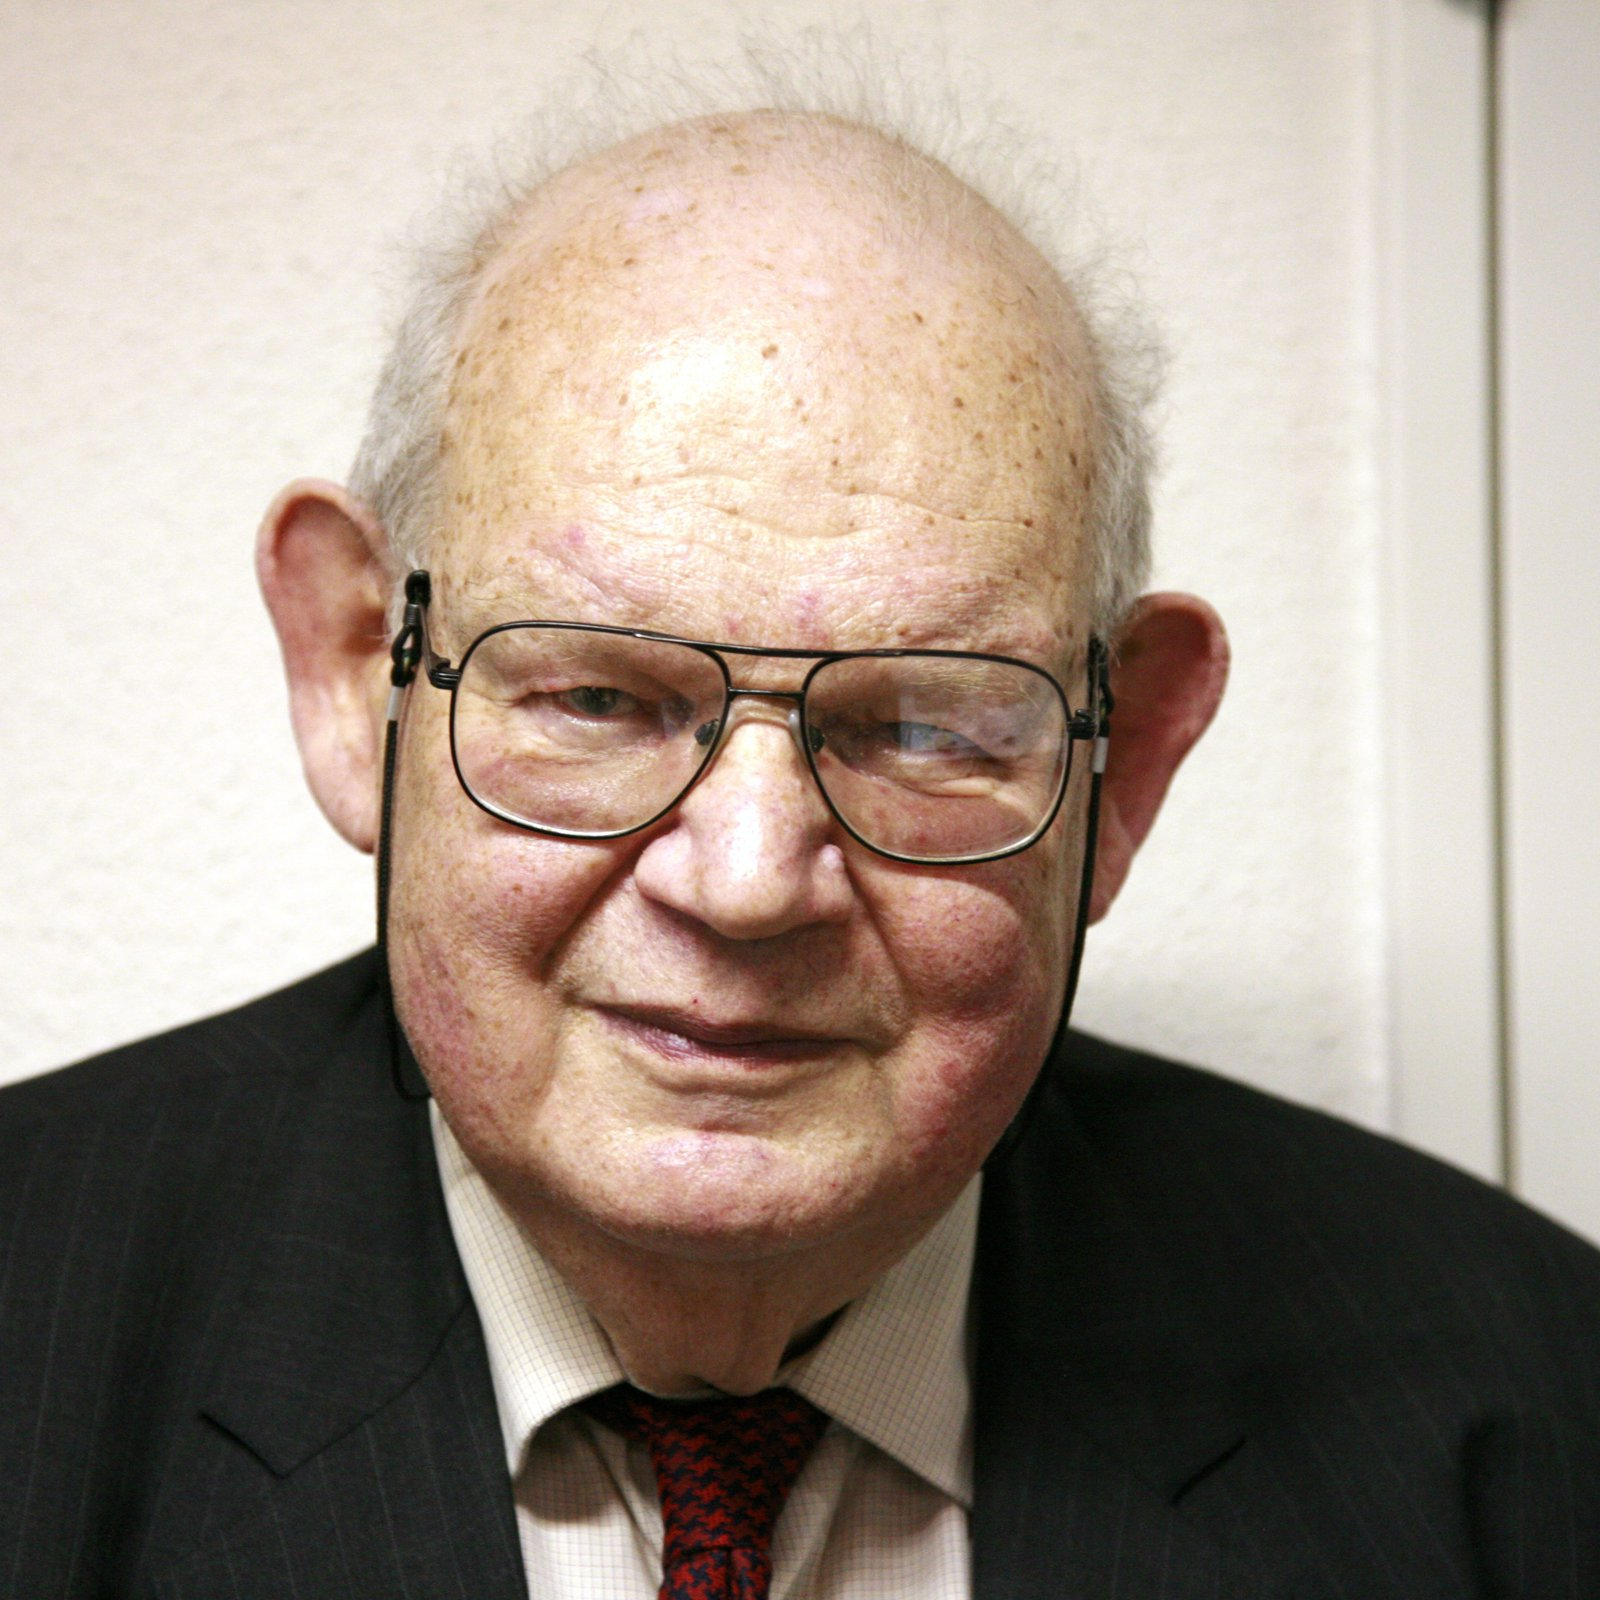
\includegraphics[height=0.40\textheight]{ch0_mandelbrot_2007.jpg}\\[1mm]
\imgcap{Benoit Mandelbrot, care a arătat în 1963 că variațiile prețurilor au cozi groase}
\imgcredit{https://commons.wikimedia.org/wiki/File:Benoit_Mandelbrot_mg_1804-d.jpg}{Foto: Rama (2007); CC BY-SA 2.0 fr; Wikimedia Commons}
\end{column}
\end{columns}
\end{frame}

\begin{frame}{Bucla de cercetare}
\itemsize{\small}
\begin{enumerate}
    \item \textbf{Întrebarea}: o frază, cu o cifră care i-ar răspunde
    \item \textbf{Datele}: seria, sursa, calendarul, fereastra, fixate înainte de a vedea rezultatele
    \item \textbf{Metoda}: testul din trusa de instrumente, cu ipoteza nulă
    \item \textbf{Verificările}: SE robuste, bandă Monte Carlo, subeșantioane, alt estimator
    \item \textbf{Interpretarea}: răspunsul, incertitudinea lui, limitele lui
    \item \textbf{Replicarea}: o a doua persoană rulează codul și obține aceleași cifre
\end{enumerate}
\begin{itemize}
    \item AI poate accelera fiecare pas; nu înlocuiește nicio verificare \refWang
\end{itemize}
\end{frame}

\begin{frame}{Contribuția posibilă a AI}
\itemsize{\small}
\begin{itemize}
    \item \textbf{Literatura}: o primă listă de studii despre eficiența și cozile piețelor emergente, fiecare verificat prin DOI
    \item \textbf{Codul}: o primă versiune a estimărilor VR(5), Hill și GARCH pe ferestre mobile de 500 de zile
    \item \textbf{Robustețea}: o grilă de alegeri (fereastra, $k$, nivelul $\alpha$, seria) și un singur tabel cu toate rezultatele
    \item \textbf{Redactarea}: un paragraf mai clar, după ce cifrele sînt finale
    \item Exemplu de prompt
    \begin{itemize}
        \item \aiprompt{Write Python code that computes, on rolling windows of 500 trading days moved by 21 days, the Lo-MacKinlay robust variance-ratio statistic Z*(5), the Hill tail index of the losses with k = 2.5\% of the window, and the GARCH(1,1)-t persistence for the daily log returns of the BET, and plots the three series with their 95\% bands.}
    \end{itemize}
\end{itemize}
\end{frame}

\begin{frame}{Verificări necesare}
\itemsize{\small}
\begin{itemize}
    \item Formulele: $Z^*(q)$ robust, nu $Z(q)$; estimatorul Hill pe pierderi $L = -r$, cu $k$ dat ca proporție din fereastră
    \item Look-ahead: fiecare fereastră folosește doar datele pînă în ultima ei zi
    \item Benzile: ferestrele suprapuse nu sînt dovezi independente; un rezultat din douăzeci este semnificativ din întîmplare
    \item Cifrele: recalculați pas cu pas o fereastră și comparați
    \item Referințele: fiecare lucrare citată trebuie să existe; deschideți DOI-ul și verificați titlul
\end{itemize}
\end{frame}

\begin{frame}{Idee de proiect}
\itemsize{\small}
\begin{itemize}
    \item \textbf{Întrebarea}: a devenit BET mai eficient, mai puțin volatil și cu cozi mai subțiri între 2000 și 2026?
    \begin{itemize}
        \item date: BET din 1997, cu S\&P 500 și DAX ca repere (EODHD)
    \end{itemize}
    \item Pași
    \begin{itemize}
        \item VR(5) robust, tail index-ul Hill, persistența GARCH și exponentul Hurst pe ferestre mobile (\sfmchlink{https://danpele.github.io/SFM/RO/Cursuri/capitol5_cozi_groase_evt.pdf}{Capitolele 5}, \sfmchlink{https://danpele.github.io/SFM/RO/Cursuri/capitol7_piete_eficiente_mers_aleator_vr.pdf}{7}, \sfmchlink{https://danpele.github.io/SFM/RO/Cursuri/capitol9_modele_arch_garch.pdf}{9}, \sfmchlink{https://danpele.github.io/SFM/RO/Cursuri/capitol11_piete_fractale_memorie_lunga.pdf}{11})
        \item benzi Monte Carlo sau bootstrap; aceeași analiză pentru repere
        \item datele de schimbare (de exemplu 2008, 2020) verificate față de benzi, nu alese după inspecția graficelor
    \end{itemize}
    \item Livrabil: un grafic cu patru panouri, un tabel și un paragraf despre ce pot și ce nu pot arăta datele
    \item Declarați orice utilizare a instrumentelor AI și enumerați erorile acestora pe care le-ați corectat
\end{itemize}
\end{frame}


%=============================================================================
\section{Rezumat}
%=============================================================================

\begin{frame}{Idei de reținut}
\itemsize{\small}
\begin{itemize}
    \item Randamente, nu prețuri: randamente logaritmice în \%, calendarul corect, anualizare cu frecvența reală
    \item Randamentele au cozi groase (tail index între 2 și 4), asimetrie negativă și varianță finită: distribuția Normală subestimează riscul
    \item Semnul randamentelor este aproape imprevizibil; mărimea lor este previzibilă (volatility clustering, GARCH)
    \item Riscul: VaR 1\% $= -q_{1\%}$ și ES 2,5\%, urmate întotdeauna de backtesting
    \item Orice rezultat are nevoie de incertitudinea lui: SE, teste robuste, benzi Monte Carlo, verificări în afara eșantionului
    \item Examenul răsplătește metoda, rezultatul și interpretarea; proiectul răsplătește o întrebare clară, cu un răspuns onest
\end{itemize}
\end{frame}

\begin{frame}{Autoevaluare}
\itemsize{\small}
\begin{itemize}
    \item \textbf{Întrebare}: Ljung--Box nu respinge pe $r_t$, dar respinge puternic pe $r_t^2$. Ce înseamnă acest lucru?
    \begin{itemize}
        \item \textbf{Răspuns}: randamentele sînt necorelate, dar nu independente: volatility clustering; modelăm varianța (GARCH)
    \end{itemize}
    \item \textbf{Întrebare}: o lege stabilă estimată dă $\hat\alpha = 1{,}5$, iar estimarea Hill este $\hat\alpha = 3$. Care are dreptate în privința varianței?
    \begin{itemize}
        \item \textbf{Răspuns}: estimarea Hill, care privește doar coada: varianța este finită; legea stabilă descrie corpul distribuției
    \end{itemize}
    \item \textbf{Întrebare}: un model are 1\% depășiri, toate în martie 2020. Este un model VaR bun?
    \begin{itemize}
        \item \textbf{Răspuns}: nu: rata este corectă, dar depășirile sînt grupate; testul Christoffersen îl respinge
    \end{itemize}
\end{itemize}
\end{frame}


%=============================================================================
\section{Bibliografie}
%=============================================================================

\begin{frame}{Bibliografie (1/2)}
\itemsize{\tiny}
\begin{itemize}
    \item Adrian, T., Brunnermeier, M.K. (2016). \href{https://doi.org/10.1257/aer.20120555}{CoVaR}. \textit{American Economic Review}, 106(7), 1705--1741.
    \item Altman, E.I. (1968). \href{https://doi.org/10.1111/j.1540-6261.1968.tb00843.x}{Financial ratios, discriminant analysis and the prediction of corporate bankruptcy}. \textit{Journal of Finance}, 23(4), 589--609.
    \item Artzner, P., Delbaen, F., Eber, J.-M., Heath, D. (1999). \href{https://doi.org/10.1111/1467-9965.00068}{Coherent measures of risk}. \textit{Mathematical Finance}, 9(3), 203--228.
    \item Bollerslev, T. (1986). \href{https://doi.org/10.1016/0304-4076(86)90063-1}{Generalized autoregressive conditional heteroskedasticity}. \textit{Journal of Econometrics}, 31(3), 307--327.
    \item Borak, S., Härdle, W.K., López-Cabrera, B. (2013). \href{https://doi.org/10.1007/978-3-642-33929-5}{\textit{Statistics of Financial Markets: Exercises and Solutions}}, 2nd ed. Springer.
    \item Campbell, J.Y., Lo, A.W., MacKinlay, A.C. (1997). \href{https://doi.org/10.1515/9781400830213}{\textit{The Econometrics of Financial Markets}}. Princeton University Press.
    \item Cont, R. (2001). \href{https://doi.org/10.1080/713665670}{Empirical properties of asset returns: stylized facts and statistical issues}. \textit{Quantitative Finance}, 1(2), 223--236.
    \item Diebold, F.X., Yilmaz, K. (2012). \href{https://doi.org/10.1016/j.ijforecast.2011.02.006}{Better to give than to receive: predictive directional measurement of volatility spillovers}. \textit{International Journal of Forecasting}, 28(1), 57--66.
    \item Engle, R.F. (1982). \href{https://doi.org/10.2307/1912773}{Autoregressive conditional heteroscedasticity with estimates of the variance of United Kingdom inflation}. \textit{Econometrica}, 50(4), 987--1007.
    \item Fama, E.F. (1970). \href{https://doi.org/10.2307/2325486}{Efficient capital markets: a review of theory and empirical work}. \textit{Journal of Finance}, 25(2), 383--417.
    \item Franke, J., Härdle, W.K., Hafner, C.M. (2019). \href{https://doi.org/10.1007/978-3-030-13751-9}{\textit{Statistics of Financial Markets: An Introduction}}, 5th ed. Springer.
    \item Gu, S., Kelly, B., Xiu, D. (2020). \href{https://doi.org/10.1093/rfs/hhaa009}{Empirical asset pricing via machine learning}. \textit{Review of Financial Studies}, 33(5), 2223--2273.
    \item Hill, B.M. (1975). \href{https://doi.org/10.1214/aos/1176343247}{A simple general approach to inference about the tail of a distribution}. \textit{Annals of Statistics}, 3(5), 1163--1174.
    \item Hurst, H.E. (1951). \href{https://doi.org/10.1061/TACEAT.0006518}{Long-term storage capacity of reservoirs}. \textit{Transactions of the American Society of Civil Engineers}, 116(1), 770--799.
    \item J.P. Morgan/Reuters (1996). \href{https://www.msci.com/documents/10199/5915b101-4206-4ba0-aee2-3449d5c7e95a}{\textit{RiskMetrics -- Technical Document}}, 4th ed. New York.
    \item Jarque, C.M., Bera, A.K. (1980). \href{https://doi.org/10.1016/0165-1765(80)90024-5}{Efficient tests for normality, homoscedasticity and serial independence of regression residuals}. \textit{Economics Letters}, 6(3), 255--259.
\end{itemize}
\end{frame}

\begin{frame}{Bibliografie (2/2)}
\itemsize{\tiny}
\begin{itemize}
    \item Kupiec, P.H. (1995). \href{https://doi.org/10.3905/jod.1995.407942}{Techniques for verifying the accuracy of risk measurement models}. \textit{Journal of Derivatives}, 3(2), 73--84.
    \item Lo, A.W., MacKinlay, A.C. (1988). \href{https://doi.org/10.1093/rfs/1.1.41}{Stock market prices do not follow random walks: evidence from a simple specification test}. \textit{Review of Financial Studies}, 1(1), 41--66.
    \item Mandelbrot, B. (1963). \href{https://doi.org/10.1086/294632}{The variation of certain speculative prices}. \textit{Journal of Business}, 36(4), 394--419.
    \item McNeil, A.J., Frey, R., Embrechts, P. (2015). \href{https://press.princeton.edu/books/hardcover/9780691166278/quantitative-risk-management}{\textit{Quantitative Risk Management: Concepts, Techniques and Tools}}, revised ed. Princeton University Press.
    \item Menkveld, A.J., Dreber, A., Holzmeister, F., Huber, J., Johannesson, M., et al. (2024). \href{https://doi.org/10.1111/jofi.13337}{Nonstandard errors}. \textit{Journal of Finance}, 79(3), 2339--2390.
    \item Nakamoto, S. (2008). \href{https://bitcoin.org/bitcoin.pdf}{Bitcoin: a peer-to-peer electronic cash system}. White paper.
    \item Nolan, J.P. (2020). \href{https://doi.org/10.1007/978-3-030-52915-4}{\textit{Univariate Stable Distributions: Models for Heavy Tailed Data}}. Springer.
    \item Peters, E.E. (1994). \href{https://www.wiley.com/en-us/Fractal+Market+Analysis\%3A+Applying+Chaos+Theory+to+Investment+and+Economics-p-9780471585244}{\textit{Fractal Market Analysis: Applying Chaos Theory to Investment and Economics}}. Wiley.
    \item Tsay, R.S. (2010). \href{https://doi.org/10.1002/9780470644560}{\textit{Analysis of Financial Time Series}}, 3rd ed. Wiley.
    \item Wang, H., Fu, T., Du, Y., Gao, W., et al. (2023). \href{https://doi.org/10.1038/s41586-023-06221-2}{Scientific discovery in the age of artificial intelligence}. \textit{Nature}, 620, 47--60.
\end{itemize}
\end{frame}

\end{document}
